%----------------------------------------------------------------------------
%----------------------------------------------------------------------------
%%%%%%%%%%%%%%%%%%%%%%%%%%%%%% -*- Mode: Latex -*- %%%%%%%%%%%%%%%%%%%%%%%%%%%%
%% >>slacT486/intro.tex<<
%% Author          : R. Jeffrey Kowalski
%% Created On      : Tue Apr 10 19:50:51 HST 2007
%% Last Modified On: Thu Aug  2 10:54:56 HST 2007
%%%%%%%%%%%%%%%%%%%%%%%%%%%%%%%%%%%%%%%%%%%%%%%%%%%%%%%%%%%%%%%%%%%%%%%%%%%%%%%
From June 19-24, 2006, the experiment, SLAC T486, was performed in the End Station A facility at the Stanford Linear Accelerator Center to measure the Askaryan effect in ice.  28.5 GeV electrons were accelerated with typically 10$^9$ particles in 10 picosecond bunches and delivered into a 7.5 metric tonne target of carving-grade ice to produce electromagnetic showers.  In a dense media like ice, coherent microwave Cherenkov radiation emerges from the particle shower and propagates to the surface of the target where radio antennas can detect the radiation.  This chapter outlines the T486 experiment and the analysis of the Askaryan effect in ice.
%----------------------------------------------------------------------------
%----------------------------------------------------------------------------
\section{Preliminary tests}
One of the simplest fundamental spectroscopy experiments is bulk absorption. Here we describe a basic absorption experiment using low cost light sources which were immediately available: light emitting diodes (LED). The LEDs response to the high voltage output of a Hg wetted relay was measured. This allowed the development of the Hg pulser system and a fast photodiode. Finally HeNe based LIF measurements are used to vet two different beam line geometries, as well as test the Hg pulser/Pockels cell system.
%----------------------------------------------------------------------------
\subsection{Broadband molecular iodine absorption}
%----------------------------------------------------------------------------
\label{LED section}
%----------------------------------------------------------------------------
\input{figures/experiments/redLED/redLED.tex}
%----------------------------------------------------------------------------
%bb defines the bounding box for the pdf
%viewport defines the area of the pdf used
%in sidewaysfigure the last entry in bb moves the caption toward/away the pic
%in sidewaysfigure the second entry in bb moves the pic toward/away the caption
%----------------------------------------------------------------------------
\begin{figure}
\scalebox{0.8}[0.8]{
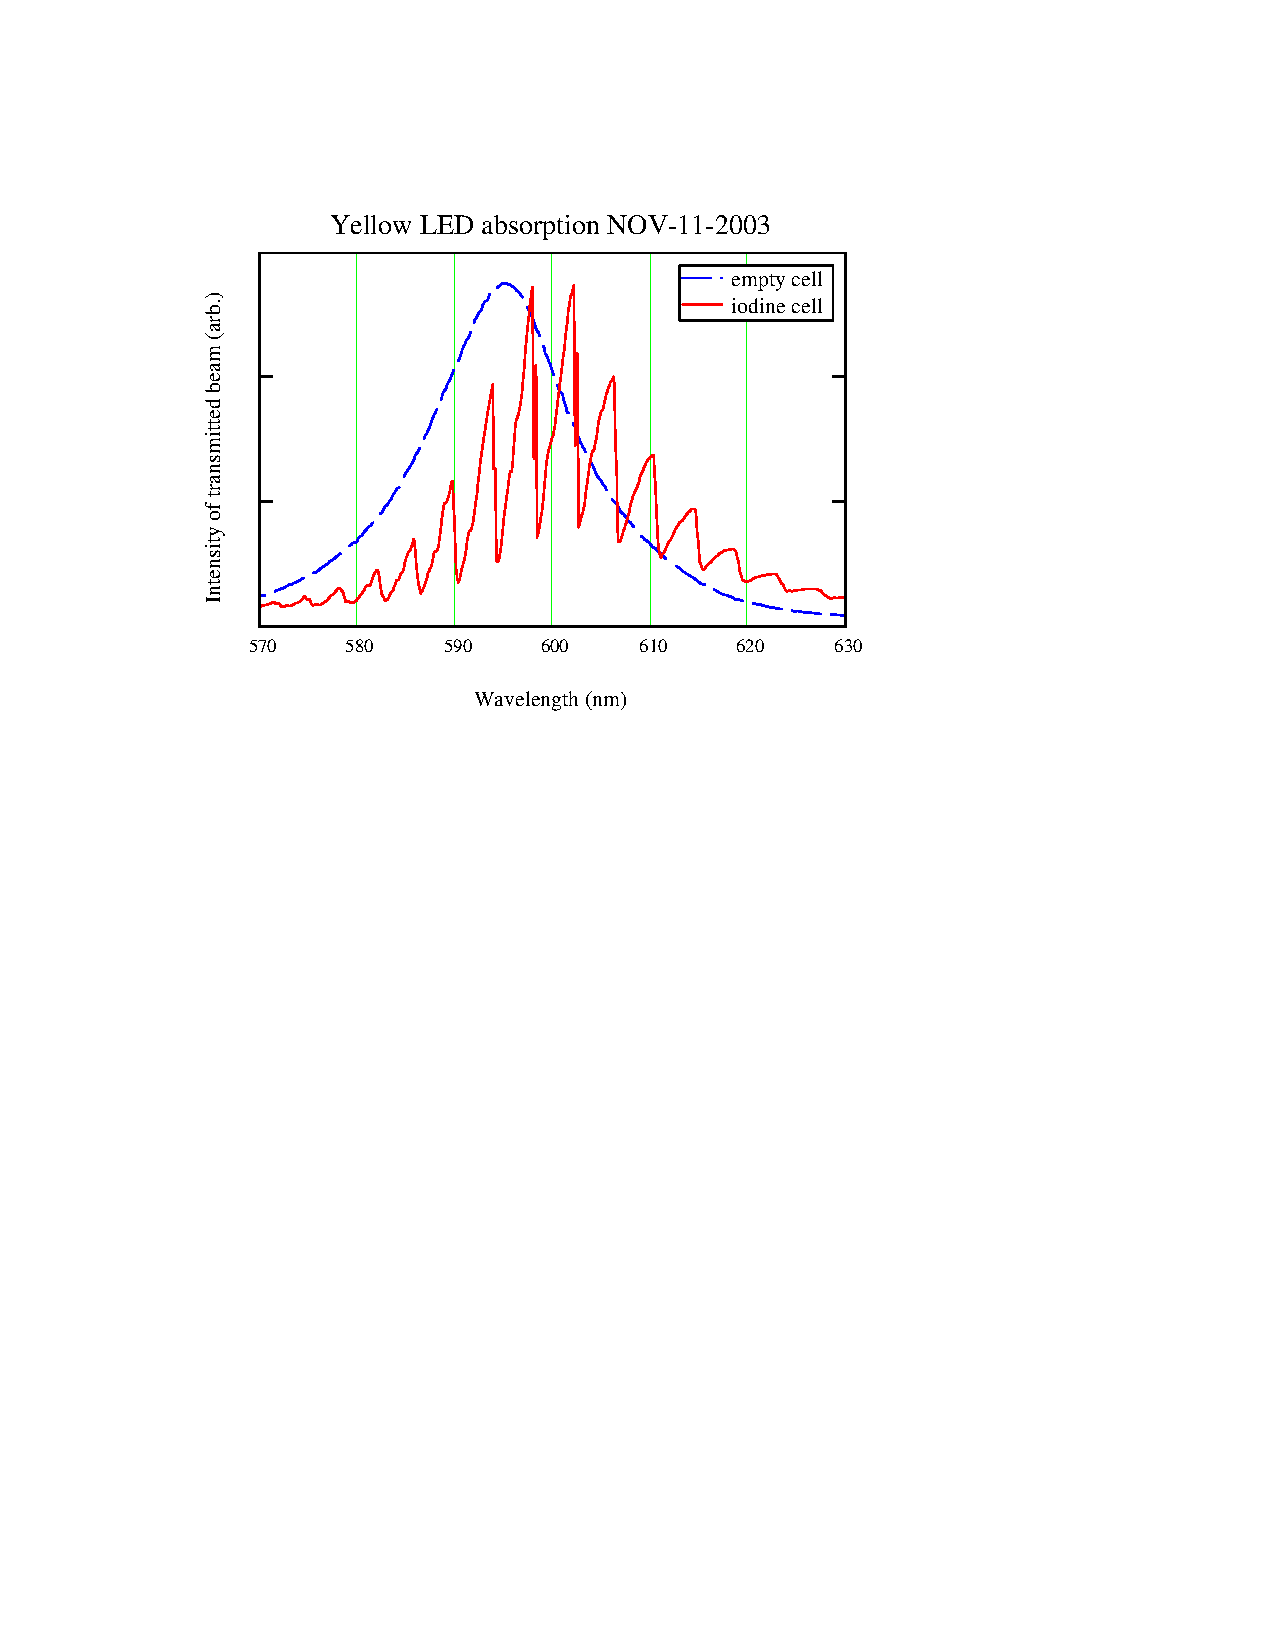
\includegraphics[bb=0 450 489 700]
{yellowLED/yellowLED.pdf}
}
\caption[Yellow LED absorption in molecular iodine]{Yellow LED absorption in molecular iodine. The solid trace is about 5 times smaller than the dashed trace}
\label{yellowLED}
\end{figure}
%----------------------------------------------------------------------------

%----------------------------------------------------------------------------
%bb defines the bounding box for the pdf
%viewport defines the area of the pdf used
%in sidewaysfigure the last entry in bb moves the caption toward/away the pic
%in sidewaysfigure the second entry in bb moves the pic toward/away the caption
%----------------------------------------------------------------------------
\begin{figure}
\scalebox{0.8}[0.8]{
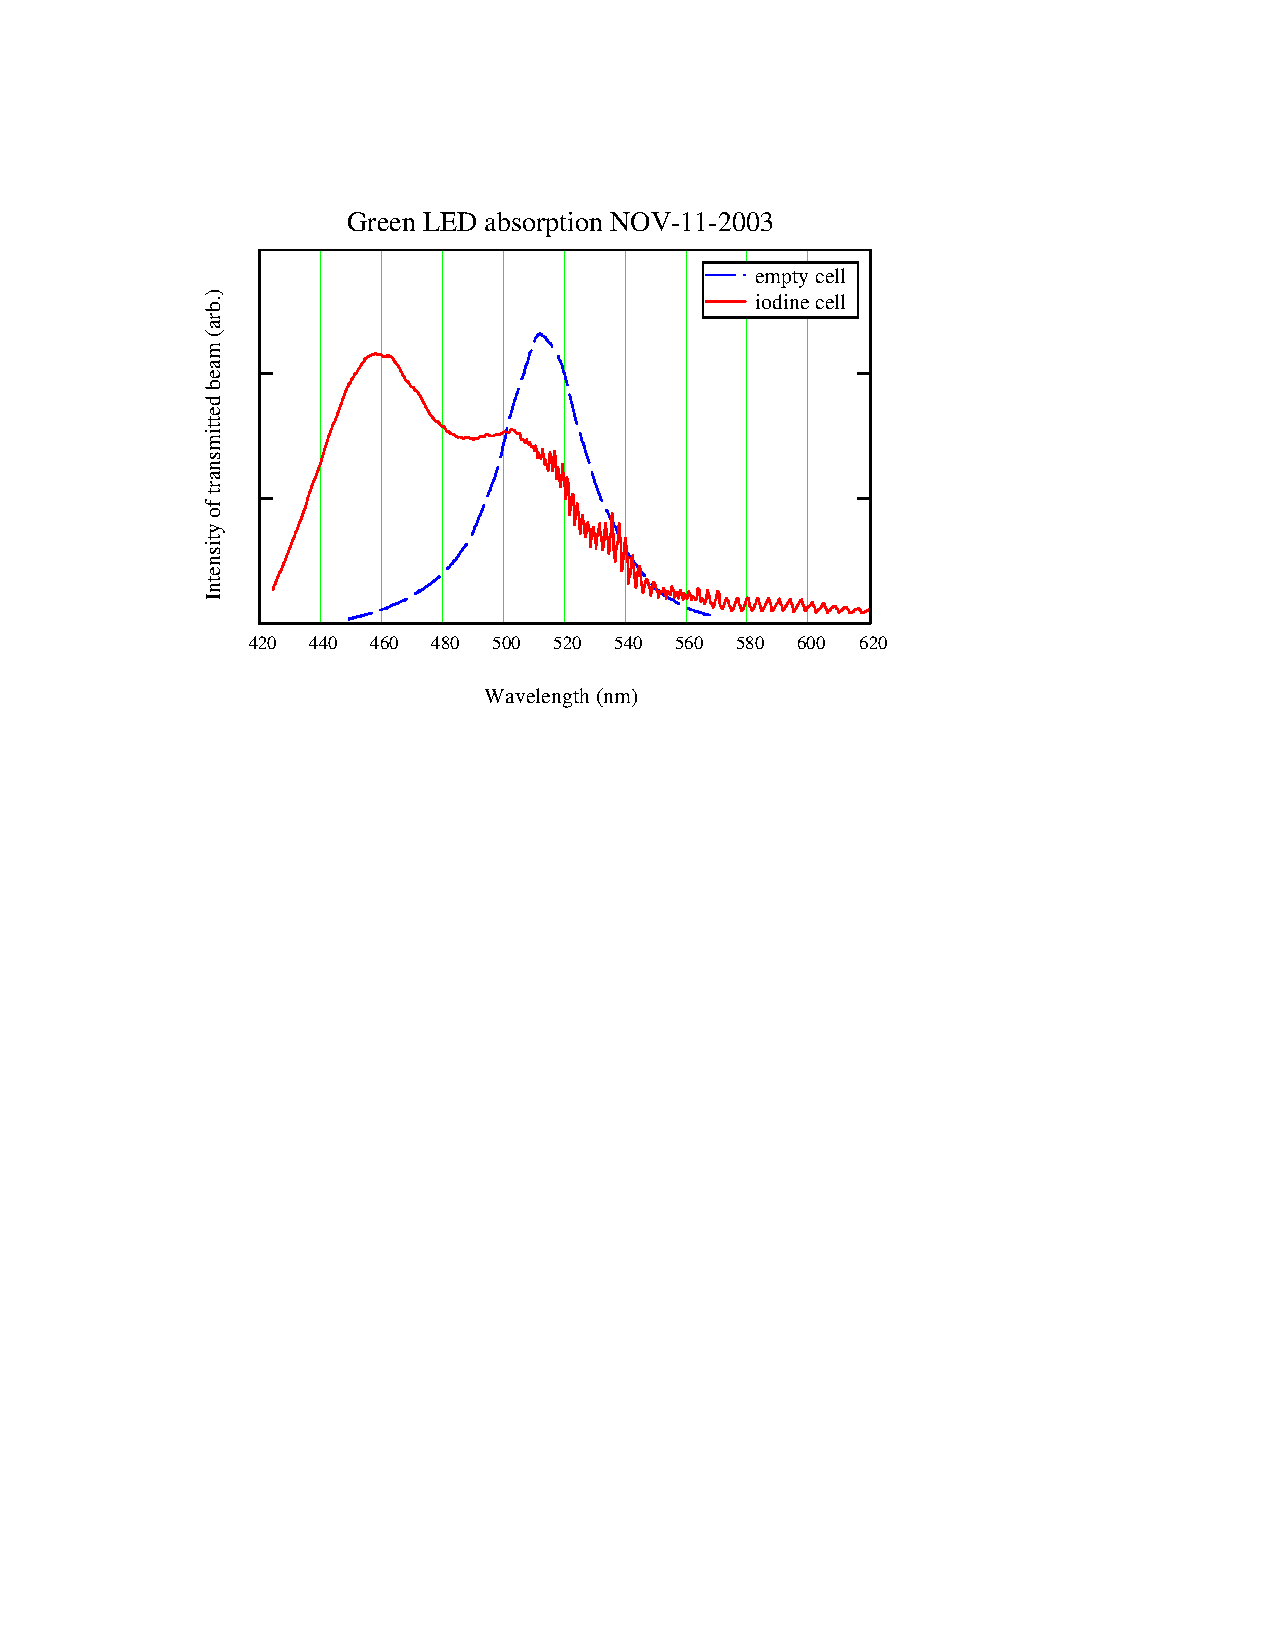
\includegraphics[bb=0 450 489 700]
{greenLED/greenLED.pdf}
}
\caption[Green LED absorption in molecular iodine]{Green LED absorption in molecular iodine. The solid trace is about 10 times smaller than the dashed trace}
\label{greenLED}
\end{figure}
%----------------------------------------------------------------------------

%----------------------------------------------------------------------------
We measure the broadband absorption spectrum of molecular iodine using LED illumination. Three LED's were used: red (see Figure \ref{redLED}), yellow (see Figure \ref{yellowLED}), green (see Figure \ref{greenLED}). The absorption features match those in the literature in shape and spectral position. Also the general observation that iodine exhibits heavier absorption in the green than the red is supported by the data.

As one of the first measurements recorded, these experiments were used to develop the essential components of this spectroscopic study: spectral analysis, light detection, data acquisition, light sources, and sample preparation. A side--view PMT is mounted at the monochromator output and encased in an aluminum foil lined cardboard box; this primitive setup proves very reliable. A chart recorder is used to acquire data; the pen axis is ``linearly'' scanned using a voltage rise from a simple RC circuit. Data processing methods are developed to account for the non-linearity of the voltage rise. Gas lamp calibration procedures are developed for use with the monochromator.

A cell is prepared in a crude fashion by simply loading a sample cell with a few flakes of iodine in an unprotected environment (outdoors, in front of the physics building), closing the cell's greased stop cock, connecting the cell to a mechanical vacuum pump, and evacuating the loaded cell at room temperature. The cell is closed off again, wrapped in heat tape, and temperature stabilized at $150^\circ$ F with a bench top controller and used on the optical bench. Ideally at this temperature the overloaded iodine cell should have a collision lifetime of 11 ns, a density of $1.9\cross10^{17}$ molecules/cm$^3$, and a pressure of 6.8 Torr (from an internal AHI document DN-3300-4 by Dr. Pui K. Lam). The cell is wrapped in aluminum foil giving it a ``baked potato'' appearance -- hereafter, this cell will be referred to as such.

%----------------------------------------------------------------------------
%----------------------------------------------------------------------------

%----------------------------------------------------------------------------
\subsection{Boxcar averager and Hg pulser}
%----------------------------------------------------------------------------
\label{Hg pulser and fast PD section}
%----------------------------------------------------------------------------
Some of the LED absorption data were taken by pulsing the LED (using an HP model 8015A pulse generator) and averaging the PMT signal with a boxcar averager (PAR, model CW--1). The goal of this experiment is to determine the usability of the donated averager; it is determined that the averager is unusable in its present state. This prompted the purchase of a new boxcar averager system.

To check the performance of a high voltage fast rise time mercury wetted relay (C.P. Clare \& Co., model HGSS 5060, called ``Hg pulser'' hereafter  -- see UH notebook UH--004 pages 49--53) and test the performance of a newly assembled fast photodiode (see UH notebook UH--015 pages 7--48), the LED's used here were connected to the output of the relay and the resulting signal observed using the fast photodiode. The relay itself is found to perform faster than the responce time of the scopes available in the lab. The LED tested can take at least 100 V in a 20 ns pulse without damage; however, it is found to have a slower response than the relay output. This may be due to the coupling between the LED and the signal cable.

%----------------------------------------------------------------------------
%----------------------------------------------------------------------------

%----------------------------------------------------------------------------
\subsection{Red and green HeNe LIF}
%----------------------------------------------------------------------------
%----------------------------------------------------------------------------
Measurements of LIF from molecular iodine illuminated with red and green HeNe can be found in the literature and are performed in undergraduate labs. We repeat some of these experiments to verify the calibration procedures to acquire spectral data and the numerical model use to analyze these data. See Figures \ref{iodine_potato} and \ref{iodine_clean} for scans of a crudely prepared iodine cell and a scan from a commercially prepared cell.
%----------------------------------------------------------------------------
%----------------------------------------------------------------------------
%bb defines the bounding box for the pdf
%viewport defines the area of the pdf used
%in sidewaysfigure the last entry in bb moves the caption toward/away the pic
%in sidewaysfigure the second entry in bb moves the pic toward/away the caption
%----------------------------------------------------------------------------
\begin{figure}
\scalebox{0.8}[0.8]{
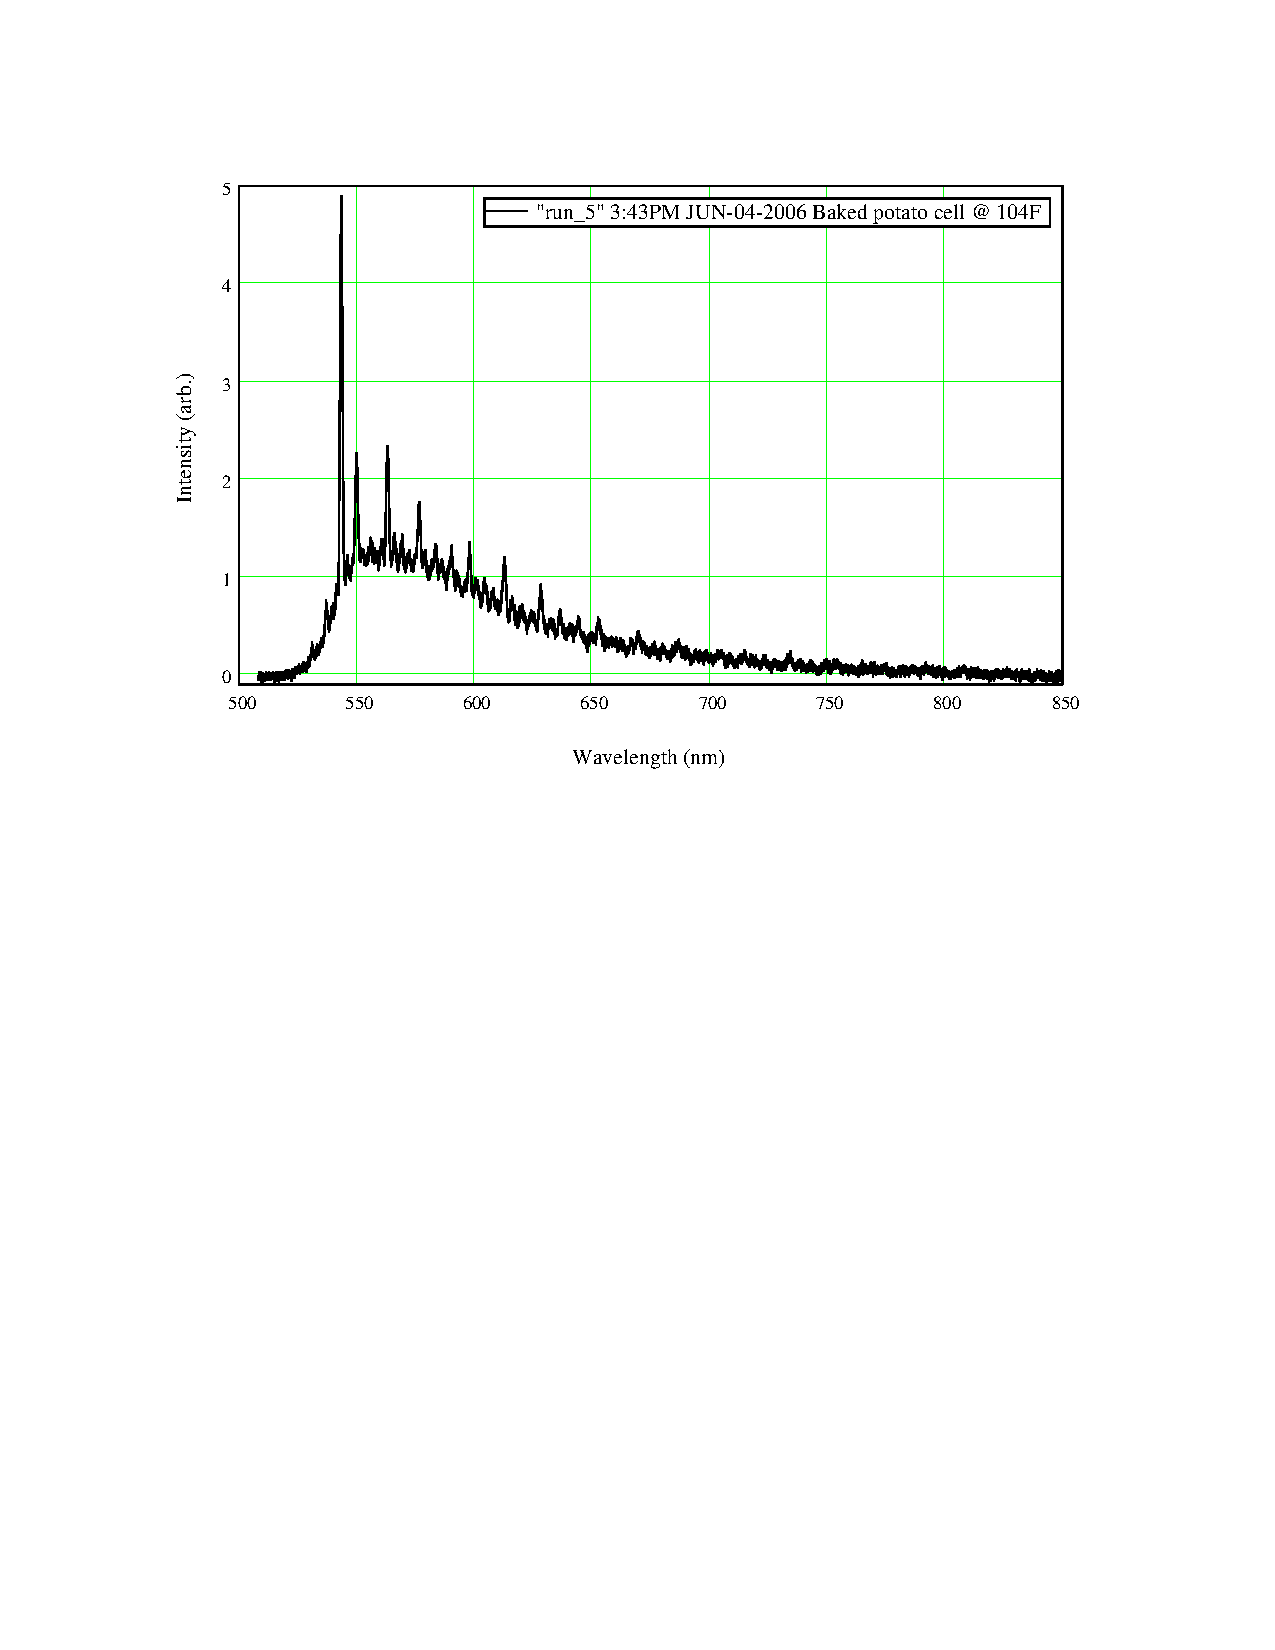
\includegraphics[bb=40 425 489 685]
{iodine_potato/iodine_potato.pdf}
}
\caption[Red HeNe LIF from the ``baked potato'' iodine cell]{Red HeNe LIF from the ``baked potato'' iodine cell. Notice the broad pedestal absent in the ``clean'' cell scan in Figure \ref{iodine_clean} -- see Section \ref{res LIF section} for discussion.}
\label{iodine_potato}
\end{figure}
%----------------------------------------------------------------------------

%----------------------------------------------------------------------------
%bb defines the bounding box for the pdf
%viewport defines the area of the pdf used
%in sidewaysfigure the last entry in bb moves the caption toward/away the pic
%in sidewaysfigure the second entry in bb moves the pic toward/away the caption
%----------------------------------------------------------------------------
\begin{figure}
\scalebox{0.8}[0.8]{
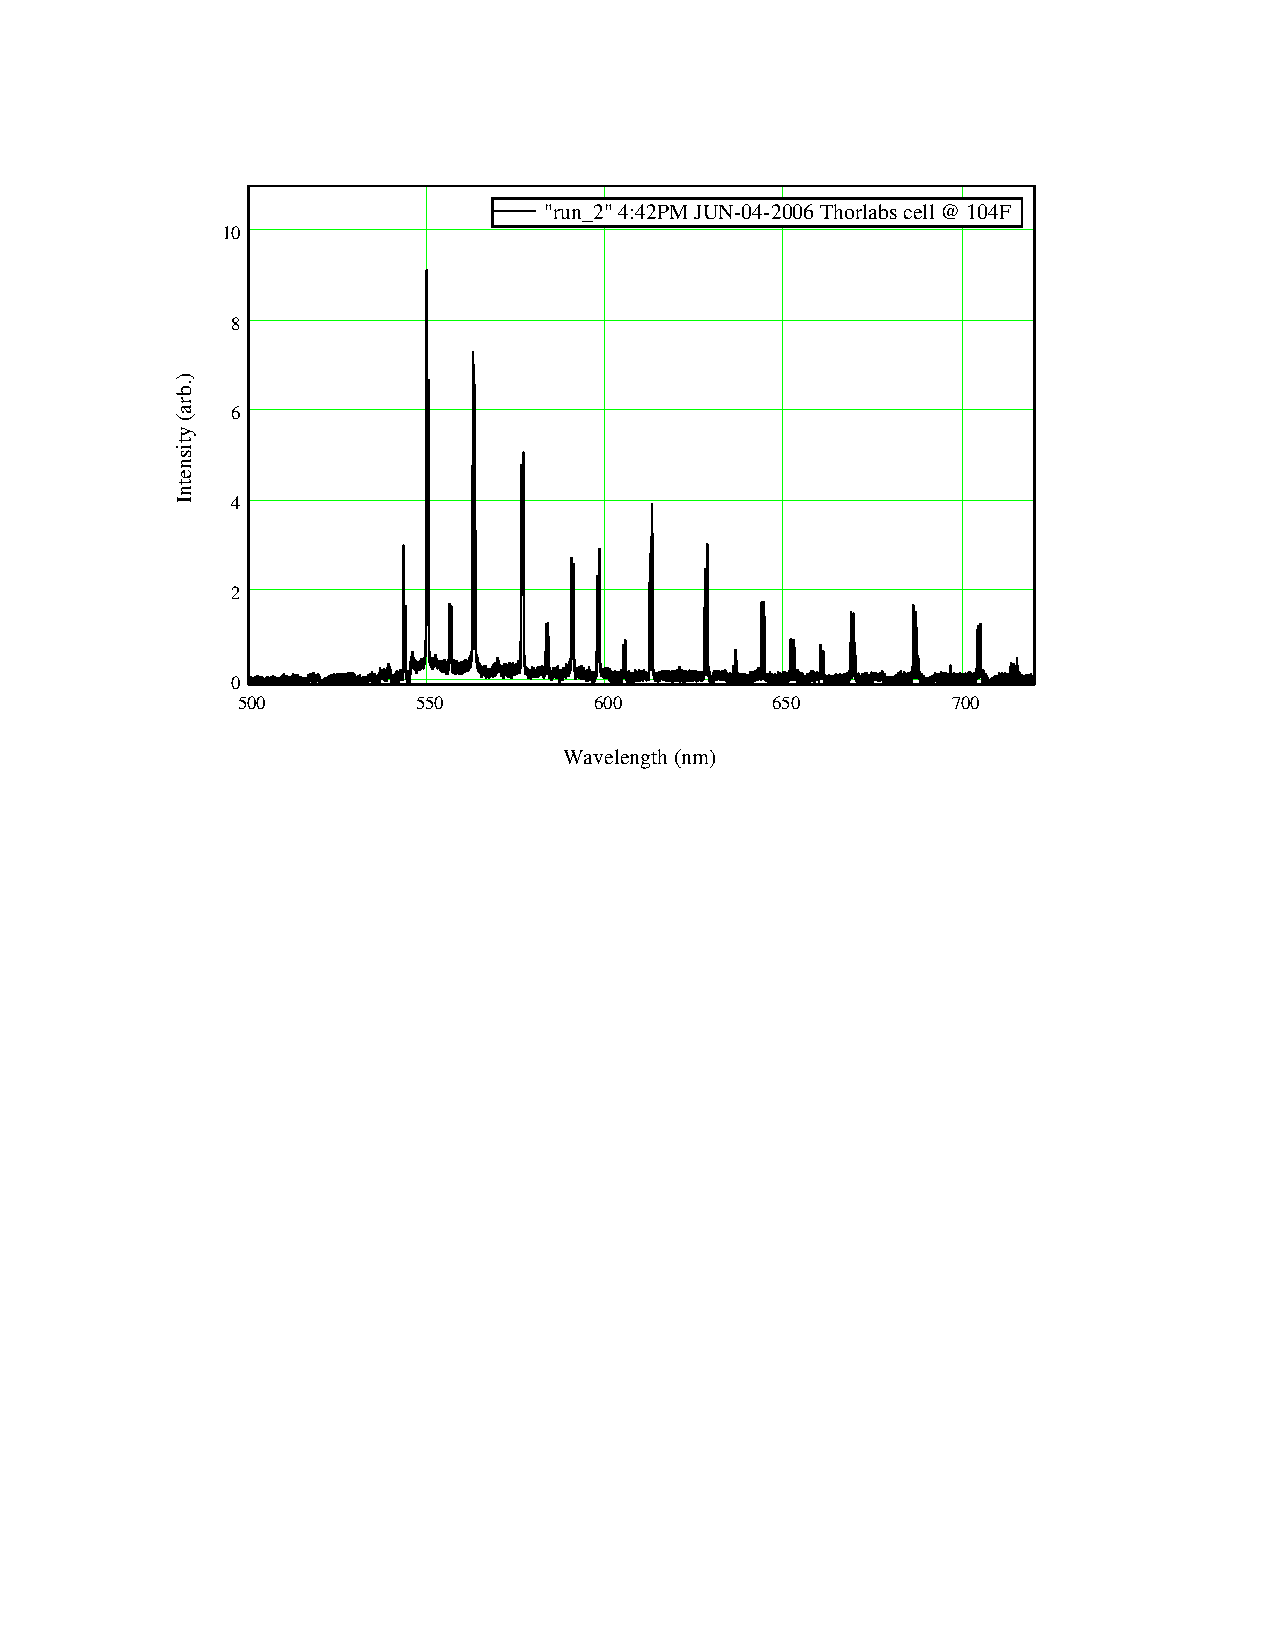
\includegraphics[bb=40 425 489 685]
{iodine_clean/iodine_clean.pdf}
}
\caption{Red HeNe LIF from a ``clean'' commercial iodine cell (Thorlabs)}
\label{iodine_clean}
\end{figure}
%----------------------------------------------------------------------------

%----------------------------------------------------------------------------

The high voltage fast rise time relay mentioned in Section \ref{Hg pulser and fast PD section} will be used to provide the fast voltage pulse that will drive the Pockels cell in the final dye laser system. The simple beam line used for the LIF measurement mentioned above is exploited to test a recently acquired Pockels cell (Cleveland Crystals Inc., Impact 8 KD*P Pockels Cell with a 532 nm AR coating). A crude Pockels cell mount is quickly constructed and the red HeNe output is sent through two crossed polarizers with the Pockels cell mounted in between. Alignment proved difficult (this knowledge prompted the design and construction of a new Pockels cell mount); however, once setup properly, the Pockels cell/Hg pulser system worked well (see Sections \ref{DC test section} and \ref{Pockels cell pulse section} or UH notebook UH--015 page 59). 
%----------------------------------------------------------------------------
%----------------------------------------------------------------------------

%----------------------------------------------------------------------------
%----------------------------------------------------------------------------
\section{Dye laser test}
This section describes three experiments mainly used to check the performance of the dye laser system (Sirah Laser model PRSC-D-24). A wavelength scanned absorption experiment reveals some problems with the mechanical systems in the dye laser. Resonant LIF from a quickly prepared cell confirms the trial molecule was a good choice and provides an opportunity to develop an automated computer based data acquisition system. Scanning the dye laser wavelength in a region containing two absorption peaks and observing the resulting fluorescence signal at high resolution reveals a subtle calibration issue and demonstrates one of the key issues in molecular discrimination: the high transition density of these systems.
%----------------------------------------------------------------------------
\subsection{Dye laser absorption in molecular iodine}
The spectral region around a targeted absorption feature is scanned in a stepwise fashion (the wavelength ``scan'' feature of the dye laser has proven unrealizable) using the ``lambdalok'' feature of the dye laser. These scans will be referenced later when we observe LIF from excitation in this region.

%------------------------------------------------------------------------------
%------------------------------------------------------------------------------
The beam line used here is similar to the one described in Section \ref{sample layout} except the attenuators are not used and in its place we use a pair of crossed polarizers (polarizing cube beam splitters) and a Pockels cell. The system has an extinction ratio of about 200:1 (see UH notebook UH-018 page 65) and produces a pulse with a FWHM of about 4 ns. Before the Pockels cell we have about 5.4 mJ, thus after the Pockels cell (heading toward the +750 mm lens) is about 27 uJ. The dye laser is tuned to 535.893 nm (a targeted absorption line) and the monochromator is tuned to capture a single LIF line at 632.9 nm. Again the signal from the PMT at the output of the monochromator is scanned (temporal gate scan) and averaged with a boxcar averager.

The measurement has facilitated the development of the data acquisition system required for lifetime measurements. The boxcar averager works at the 1000 ps gate width setting (it has settings down to 100 ps, but these have not been tried) and the LabView program records the data as a convenient text file. We have also discovered that the intensity fluctuations of the dye laser output introduce unwanted jitter in the position of the trigger relative to the peak -- accurate lifetime measurements will require a way to eliminate the jitter or, better yet, reduce the intensity fluctuations in the input beam. Contamination of the cell may have introduced additional channels through which the iodine can decay. A clean loading method must be developed in order to isolate and measure specific effects on the fluorescence decay.
%------------------------------------------------------------------------------
%------------------------------------------------------------------------------
%------------------------------------------------------------------------------
%------------------------------------------------------------------------------
%------------------------------------------------------------------------------
%------------------------------------------------------------------------------


%----------------------------------------------------------------------------
%----------------------------------------------------------------------------
%----------------------------------------------------------------------------
%bb defines the bounding box for the pdf
%viewport defines the area of the pdf used
%in sidewaysfigure the last entry in bb moves the caption toward/away the pic
%in sidewaysfigure the second entry in bb moves the pic toward/away the caption
%----------------------------------------------------------------------------
\begin{figure}
\scalebox{0.8}[0.8]{
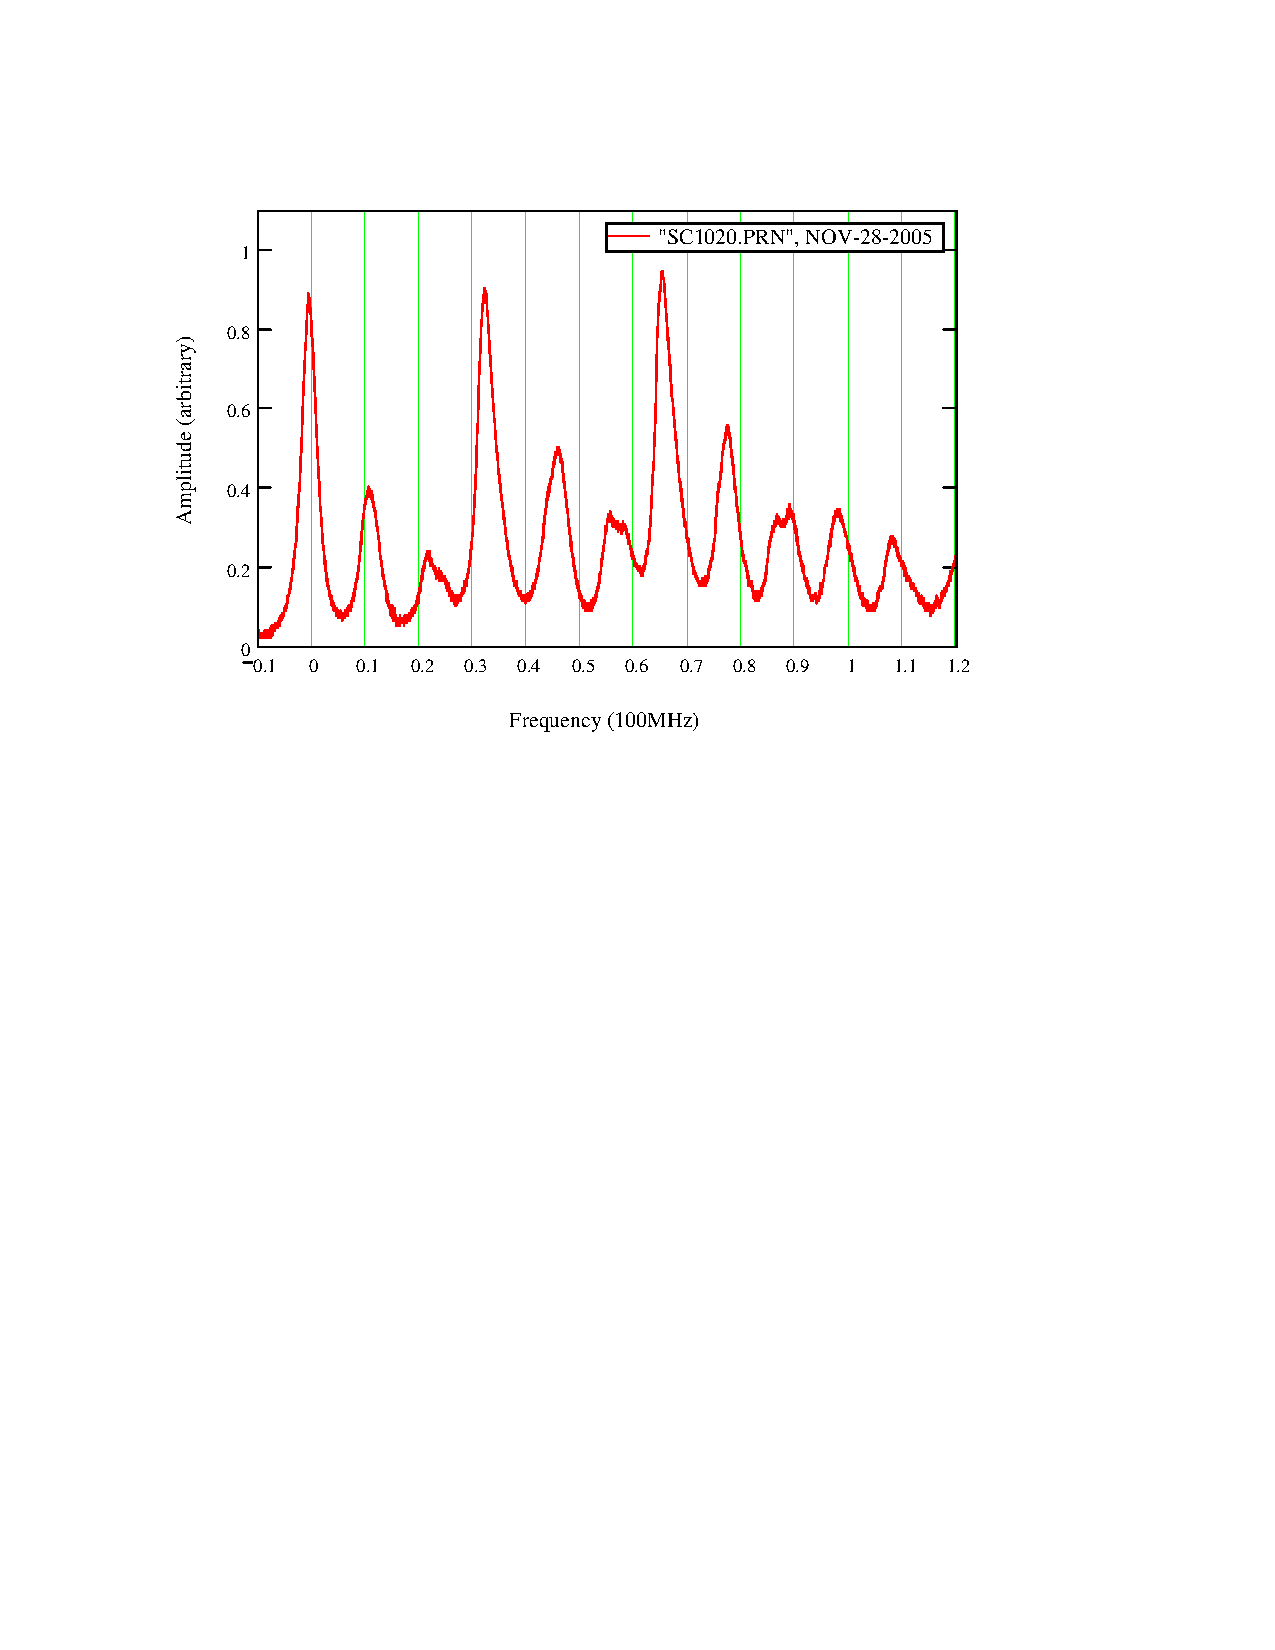
\includegraphics[bb=15 440 489 752]
{near_confocal/near_confocal.pdf}
}
\caption[Green HeNe transmission through a scaned near confocal etalon]{Green HeNe transmission through a scaned near confocal etalon}
\label{near_confocal}
\end{figure}
%----------------------------------------------------------------------------

%----------------------------------------------------------------------------
%----------------------------------------------------------------------------
%bb defines the bounding box for the pdf
%viewport defines the area of the pdf used
%in sidewaysfigure the last entry in bb moves the caption toward/away the pic
%in sidewaysfigure the second entry in bb moves the pic toward/away the caption
%----------------------------------------------------------------------------
\begin{figure}
\scalebox{0.8}[0.8]{
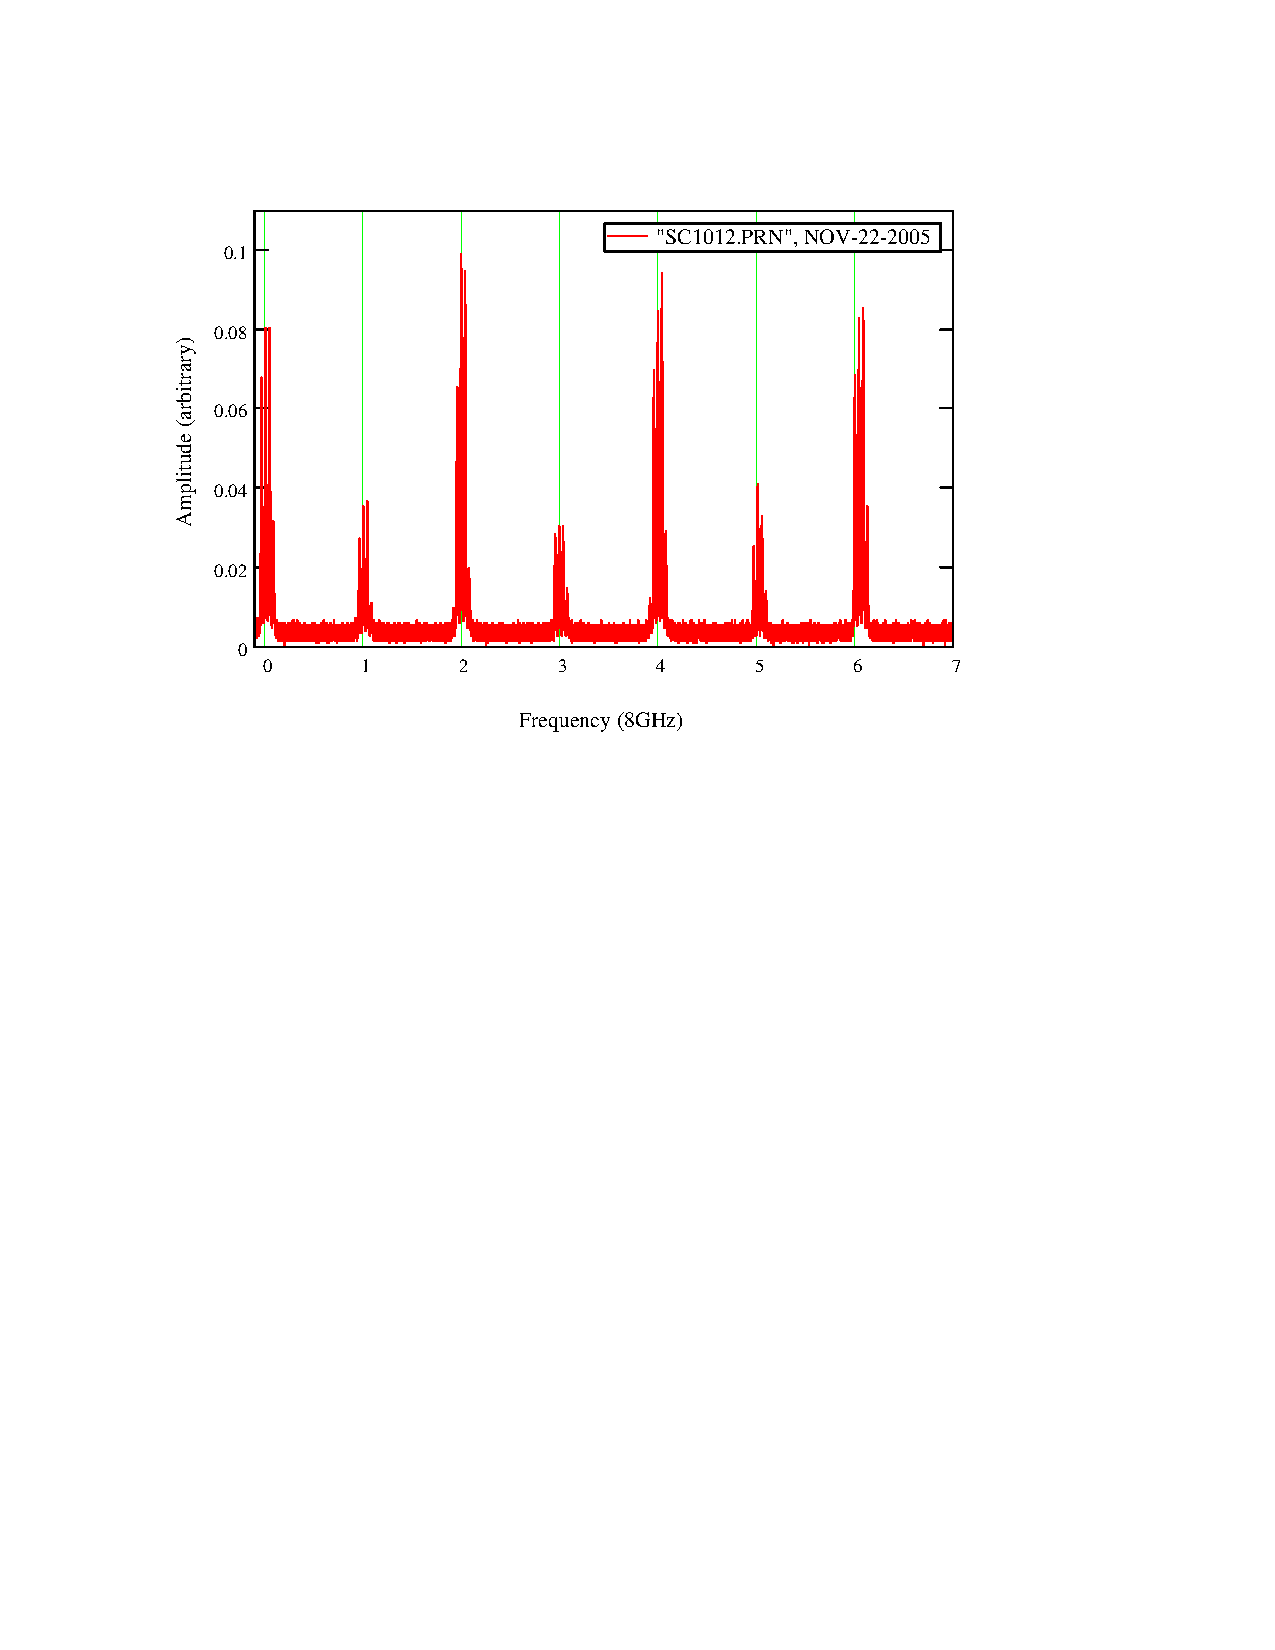
\includegraphics[bb=15 440 489 752]
{confocal_all/confocal_all.pdf}
}
\caption[Green HeNe transmission through a scanned confocal etalon]{Green HeNe transmission through a scanned confocal etalon}
\label{confocal_all}
\end{figure}
%----------------------------------------------------------------------------

%----------------------------------------------------------------------------
%----------------------------------------------------------------------------
%bb defines the bounding box for the pdf
%viewport defines the area of the pdf used
%in sidewaysfigure the last entry in bb moves the caption toward/away the pic
%in sidewaysfigure the second entry in bb moves the pic toward/away the caption
%----------------------------------------------------------------------------
\begin{figure}
\scalebox{0.8}[0.8]{
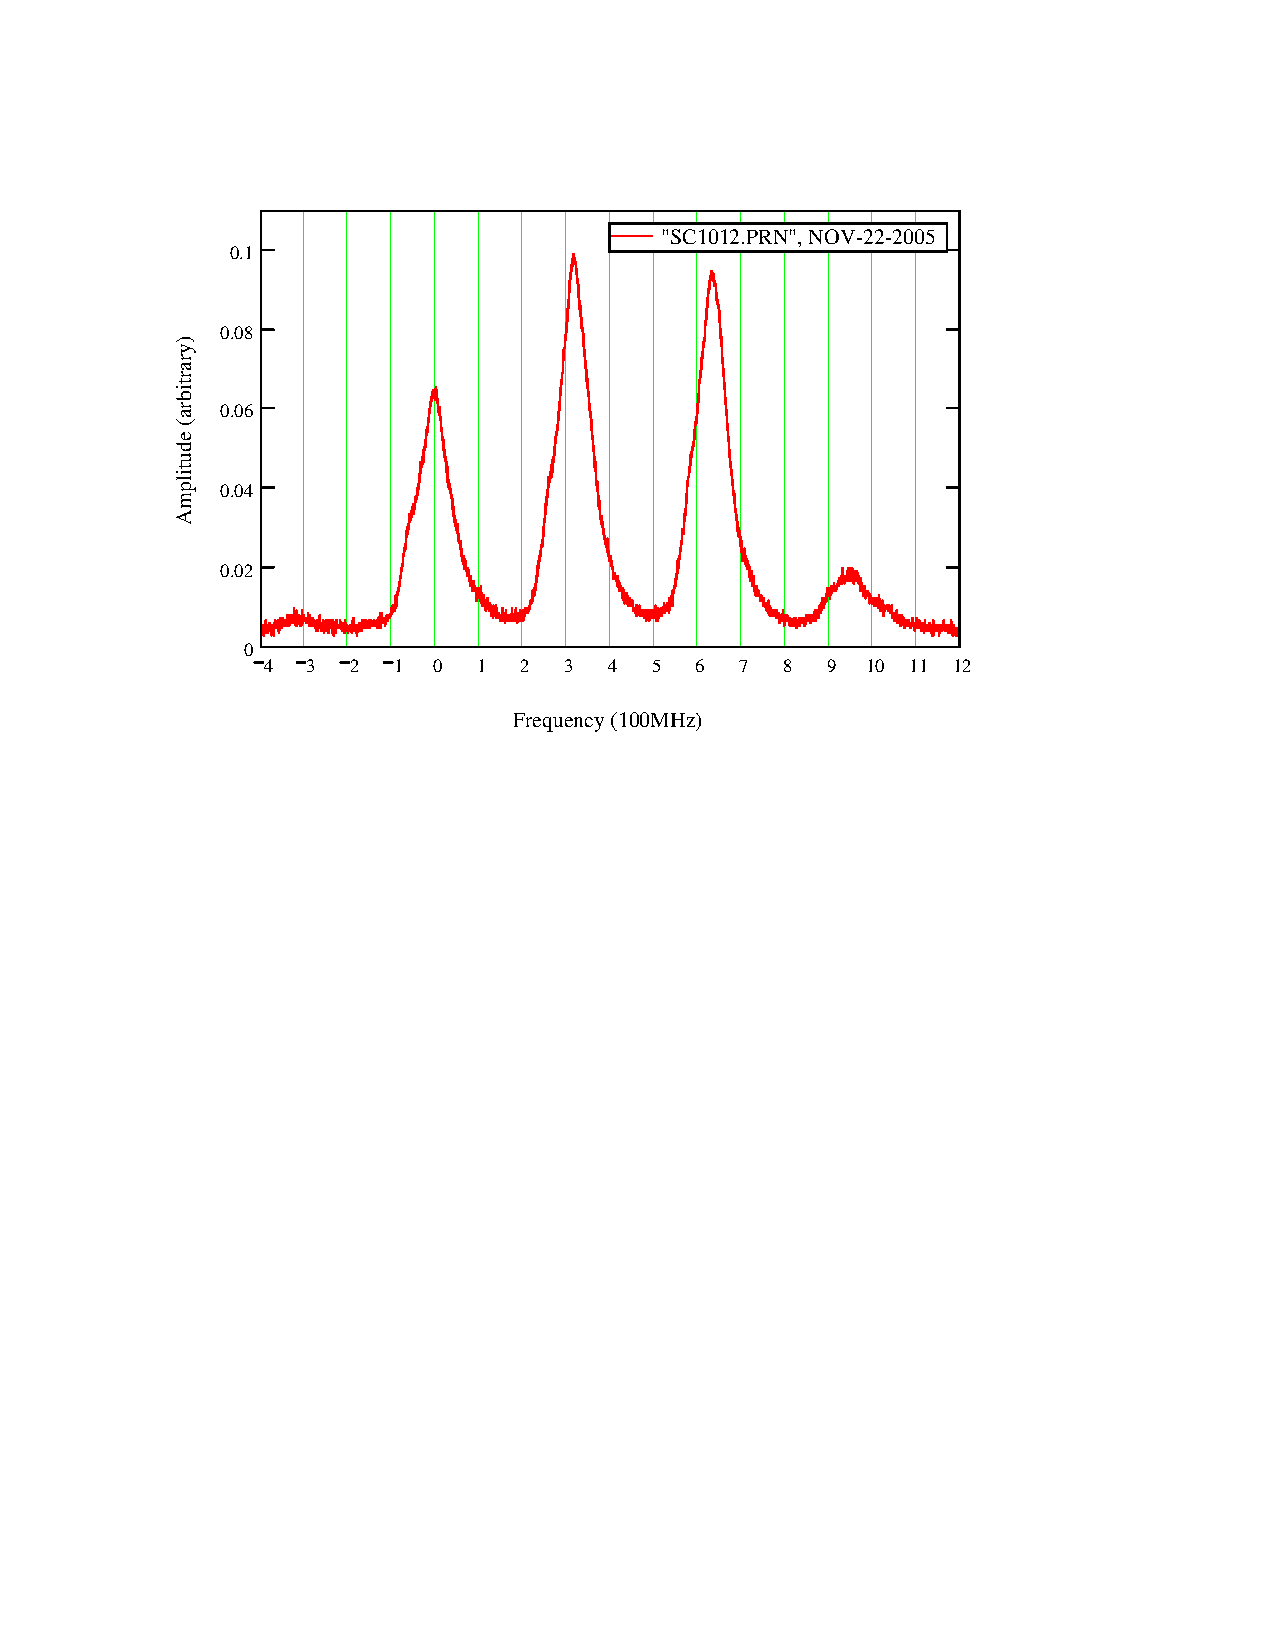
\includegraphics[bb=15 440 489 752]
{confocal_zoom/confocal_zoom.pdf}
}
\caption[Green HeNe transmission through a scanned confocal etalon (zoom)]{Green HeNe transmission through a scanned confocal etalon (zoom). The green HeNe mode spacing is 326 MHz and the etalon mode width is 100 MHz.}
\label{confocal_zoom}
\end{figure}
%----------------------------------------------------------------------------

%----------------------------------------------------------------------------
%----------------------------------------------------------------------------

%----------------------------------------------------------------------------
%----------------------------------------------------------------------------
\subsection{Resonant laser induced fluroescence}
\label{res LIF section}
%------------------------------------------------------------------------------
%------------------------------------------------------------------------------
The beam line used here is similar to the one described in Section \ref{sample layout} except the attenuators are not used and in its place we use a pair of crossed polarizers (polarizing cube beam splitters) and a Pockels cell. The system has an extinction ratio of about 200:1 (see UH notebook UH-018 page 65) and produces a pulse with a FWHM of about 4 ns. Before the Pockels cell we have about 5.4 mJ, thus after the Pockels cell (heading toward the +750 mm lens) is about 27 uJ. The dye laser is tuned to 535.893 nm (a targeted absorption line) and the monochromator is tuned to capture a single LIF line at 632.9 nm. Again the signal from the PMT at the output of the monochromator is scanned (temporal gate scan) and averaged with a boxcar averager.

The measurement has facilitated the development of the data acquisition system required for lifetime measurements. The boxcar averager works at the 1000 ps gate width setting (it has settings down to 100 ps, but these have not been tried) and the LabView program records the data as a convenient text file. We have also discovered that the intensity fluctuations of the dye laser output introduce unwanted jitter in the position of the trigger relative to the peak -- accurate lifetime measurements will require a way to eliminate the jitter or, better yet, reduce the intensity fluctuations in the input beam. Contamination of the cell may have introduced additional channels through which the iodine can decay. A clean loading method must be developed in order to isolate and measure specific effects on the fluorescence decay.
%------------------------------------------------------------------------------
%------------------------------------------------------------------------------
%------------------------------------------------------------------------------
%------------------------------------------------------------------------------
%------------------------------------------------------------------------------
%------------------------------------------------------------------------------


%----------------------------------------------------------------------------
%----------------------------------------------------------------------------
%----------------------------------------------------------------------------
%bb defines the bounding box for the pdf
%viewport defines the area of the pdf used
%in sidewaysfigure the last entry in bb moves the caption toward/away the pic
%in sidewaysfigure the second entry in bb moves the pic toward/away the caption
%----------------------------------------------------------------------------
\begin{figure}
\scalebox{0.8}[0.8]{
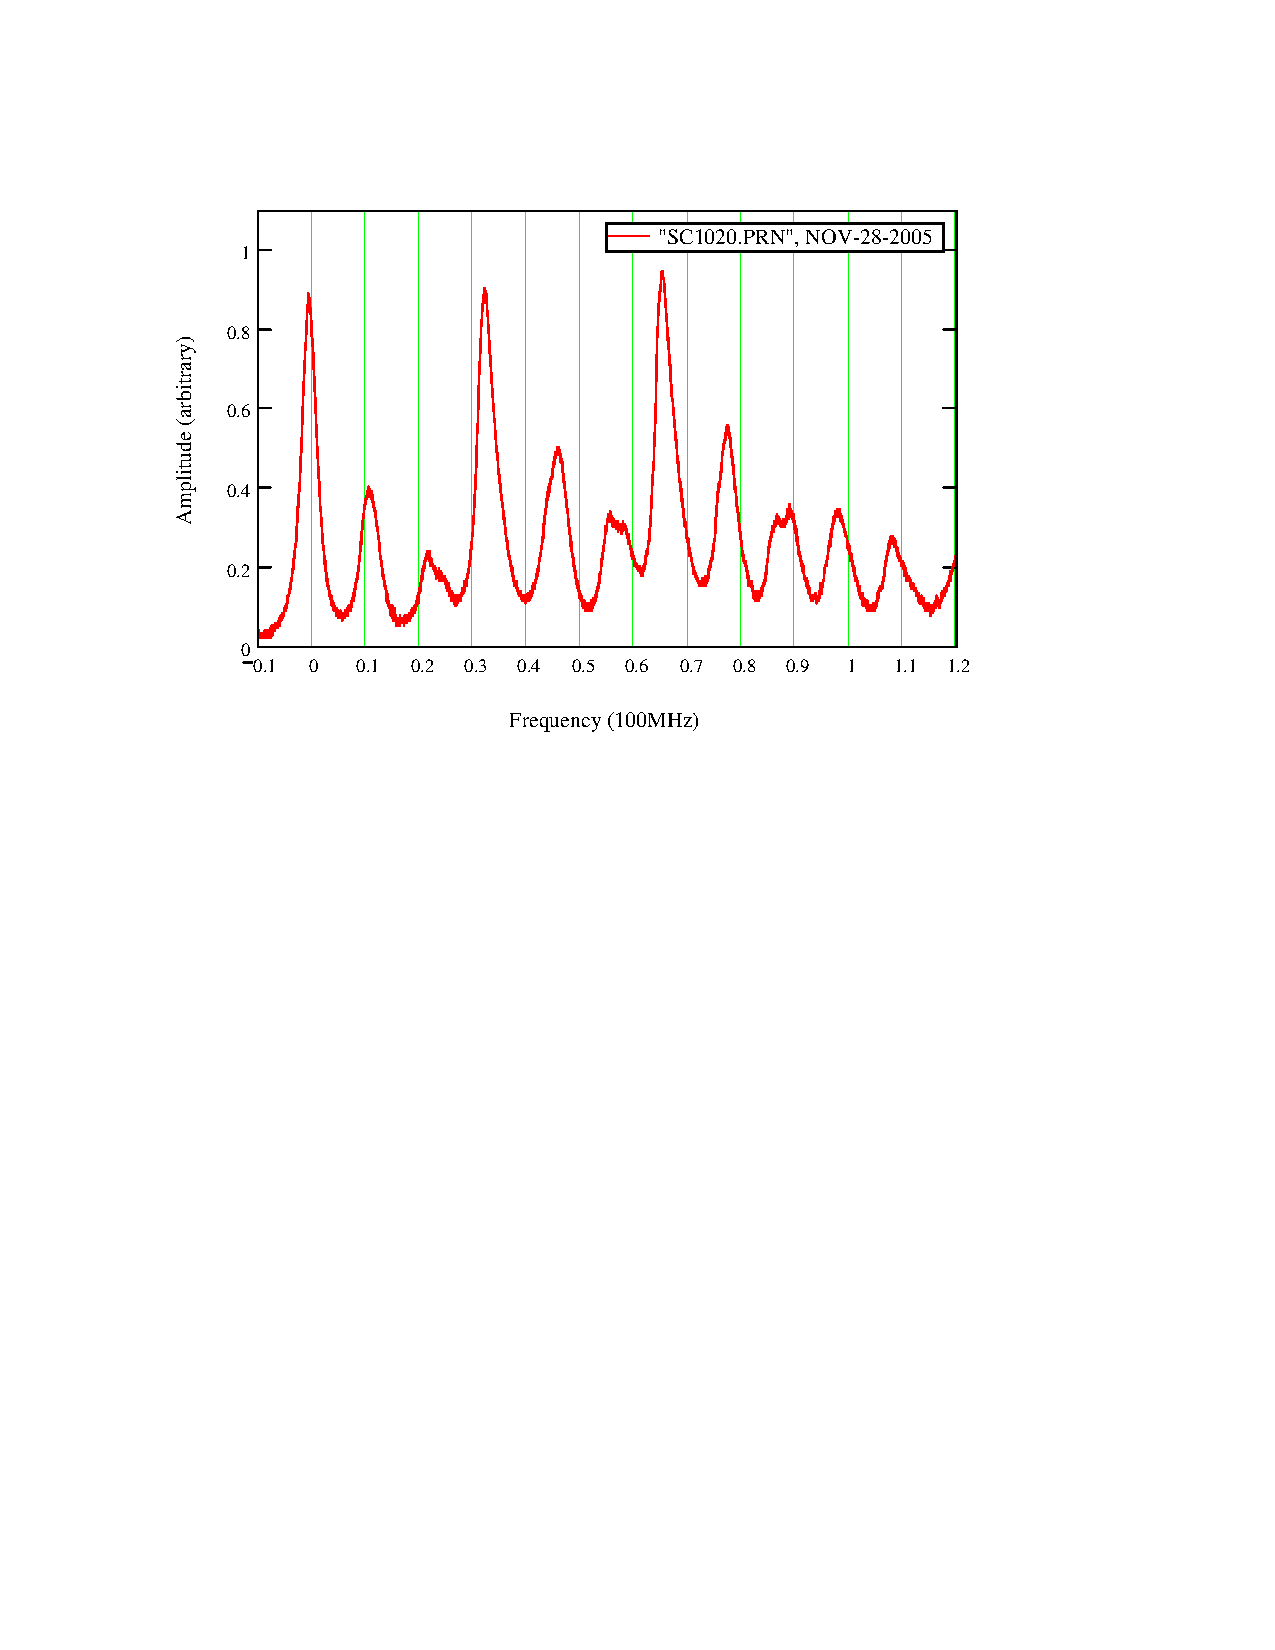
\includegraphics[bb=15 440 489 752]
{near_confocal/near_confocal.pdf}
}
\caption[Green HeNe transmission through a scaned near confocal etalon]{Green HeNe transmission through a scaned near confocal etalon}
\label{near_confocal}
\end{figure}
%----------------------------------------------------------------------------

%----------------------------------------------------------------------------
%----------------------------------------------------------------------------
%bb defines the bounding box for the pdf
%viewport defines the area of the pdf used
%in sidewaysfigure the last entry in bb moves the caption toward/away the pic
%in sidewaysfigure the second entry in bb moves the pic toward/away the caption
%----------------------------------------------------------------------------
\begin{figure}
\scalebox{0.8}[0.8]{
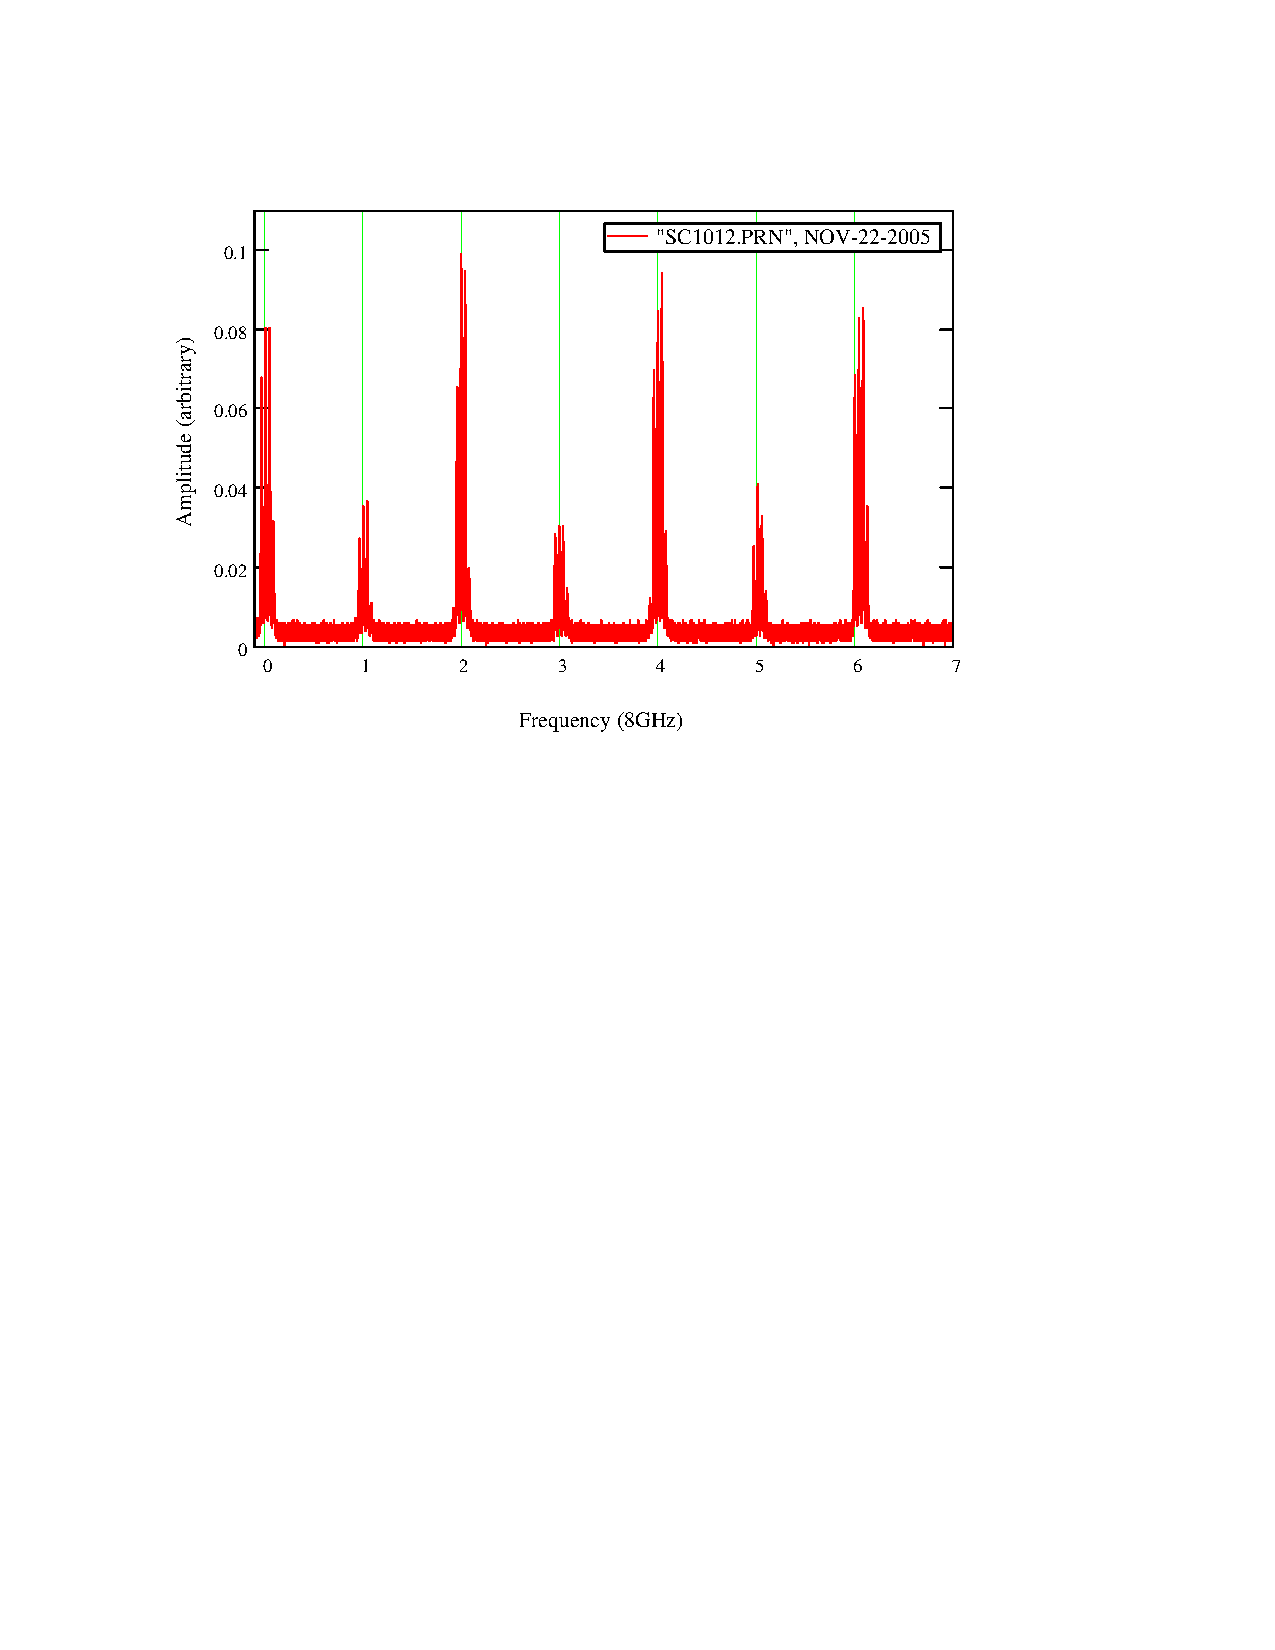
\includegraphics[bb=15 440 489 752]
{confocal_all/confocal_all.pdf}
}
\caption[Green HeNe transmission through a scanned confocal etalon]{Green HeNe transmission through a scanned confocal etalon}
\label{confocal_all}
\end{figure}
%----------------------------------------------------------------------------

%----------------------------------------------------------------------------
%----------------------------------------------------------------------------
%bb defines the bounding box for the pdf
%viewport defines the area of the pdf used
%in sidewaysfigure the last entry in bb moves the caption toward/away the pic
%in sidewaysfigure the second entry in bb moves the pic toward/away the caption
%----------------------------------------------------------------------------
\begin{figure}
\scalebox{0.8}[0.8]{
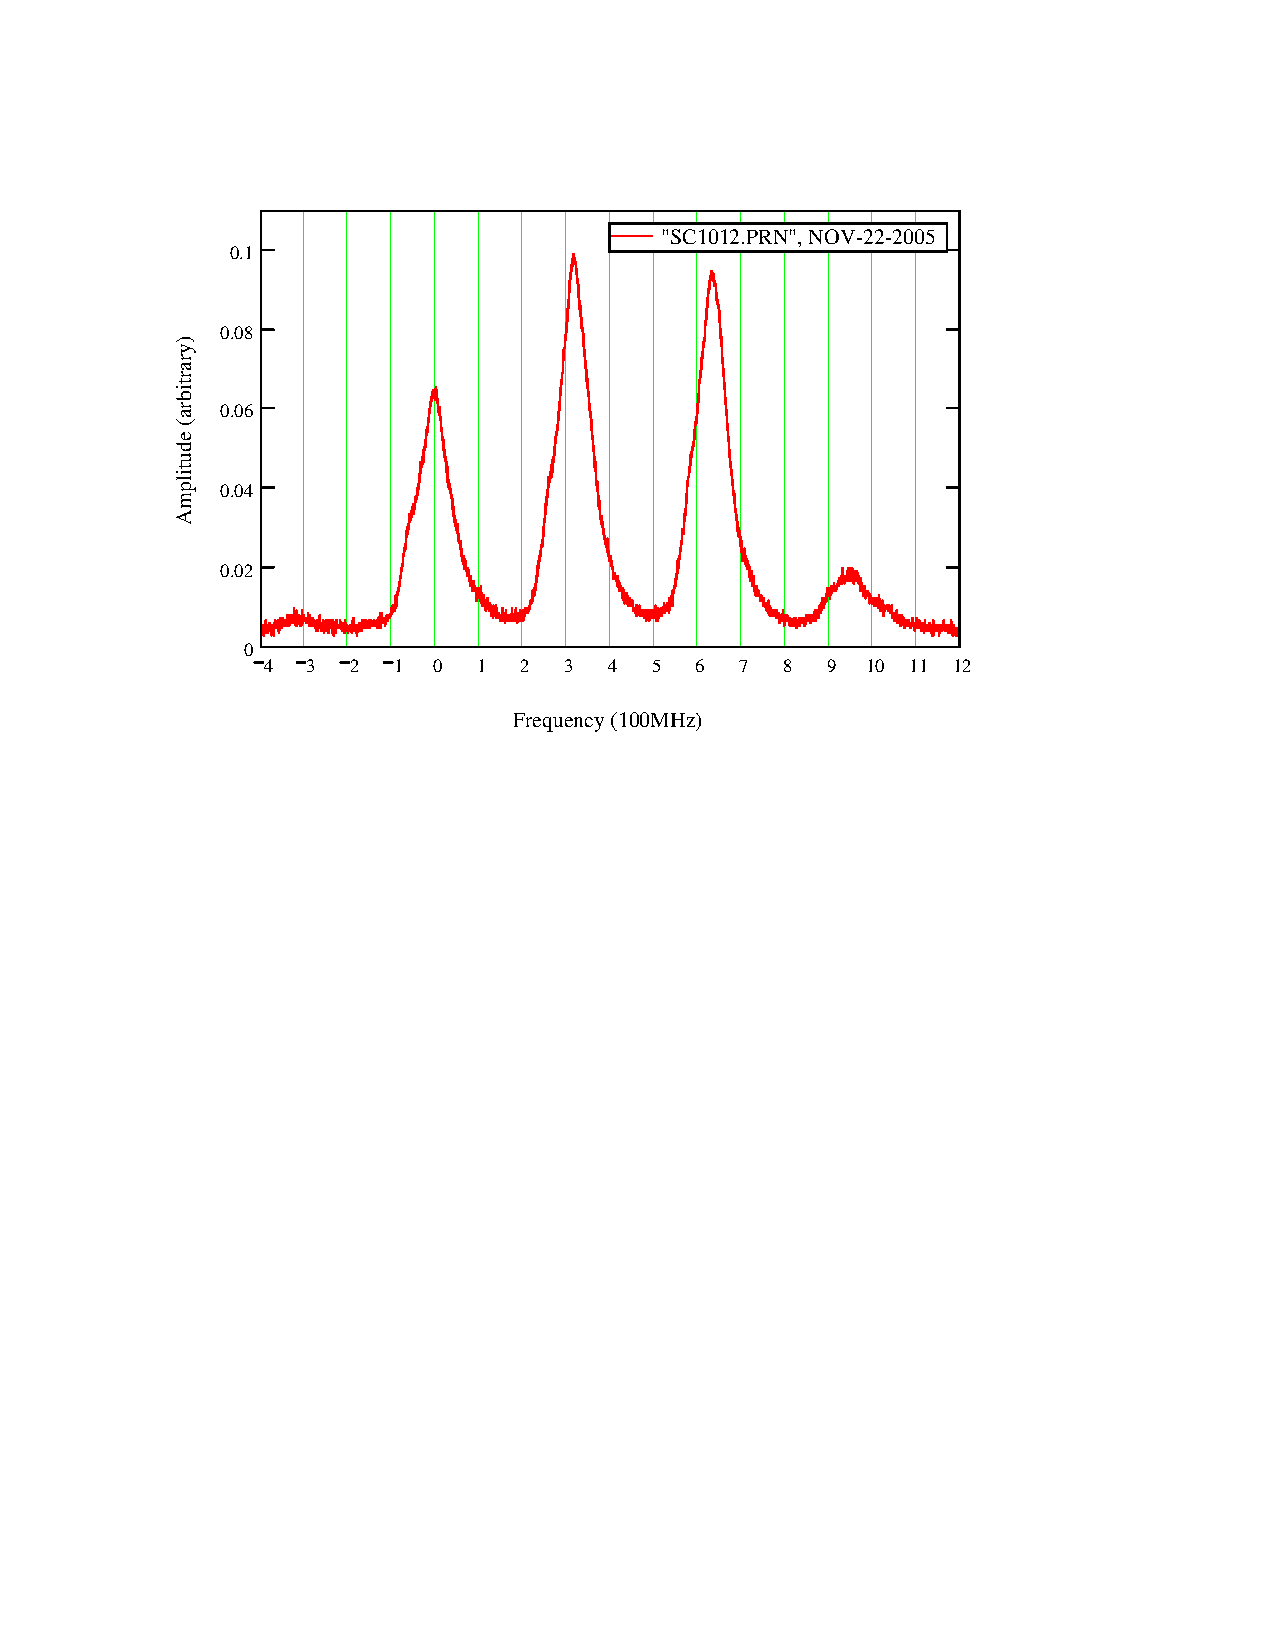
\includegraphics[bb=15 440 489 752]
{confocal_zoom/confocal_zoom.pdf}
}
\caption[Green HeNe transmission through a scanned confocal etalon (zoom)]{Green HeNe transmission through a scanned confocal etalon (zoom). The green HeNe mode spacing is 326 MHz and the etalon mode width is 100 MHz.}
\label{confocal_zoom}
\end{figure}
%----------------------------------------------------------------------------

%----------------------------------------------------------------------------
%----------------------------------------------------------------------------

%----------------------------------------------------------------------------
%----------------------------------------------------------------------------
\subsection{Transition selection}
The dye laser system maintains enough control of its output spectrum to allow discrimination between a target transition and its nearest strong neighbor. There may be some remaining calibration issues, but the numerical model for iodine LIF does a good job of modeling the observed spectral features in the LIF spectrum. Transition one and two (see Section \ref{absorption data section}) are selected by tuning the dye laser to their respective wavelengths and the resulting fluorescence spectra are observed.

%------------------------------------------------------------------------------
%------------------------------------------------------------------------------
The beam line used here is similar to the one described in Section \ref{sample layout} except the attenuators are not used and in its place we use a pair of crossed polarizers (polarizing cube beam splitters) and a Pockels cell. The system has an extinction ratio of about 200:1 (see UH notebook UH-018 page 65) and produces a pulse with a FWHM of about 4 ns. Before the Pockels cell we have about 5.4 mJ, thus after the Pockels cell (heading toward the +750 mm lens) is about 27 uJ. The dye laser is tuned to 535.893 nm (a targeted absorption line) and the monochromator is tuned to capture a single LIF line at 632.9 nm. Again the signal from the PMT at the output of the monochromator is scanned (temporal gate scan) and averaged with a boxcar averager.

The measurement has facilitated the development of the data acquisition system required for lifetime measurements. The boxcar averager works at the 1000 ps gate width setting (it has settings down to 100 ps, but these have not been tried) and the LabView program records the data as a convenient text file. We have also discovered that the intensity fluctuations of the dye laser output introduce unwanted jitter in the position of the trigger relative to the peak -- accurate lifetime measurements will require a way to eliminate the jitter or, better yet, reduce the intensity fluctuations in the input beam. Contamination of the cell may have introduced additional channels through which the iodine can decay. A clean loading method must be developed in order to isolate and measure specific effects on the fluorescence decay.
%------------------------------------------------------------------------------
%------------------------------------------------------------------------------
%------------------------------------------------------------------------------
%------------------------------------------------------------------------------
%------------------------------------------------------------------------------
%------------------------------------------------------------------------------


%----------------------------------------------------------------------------
%----------------------------------------------------------------------------
%----------------------------------------------------------------------------
%bb defines the bounding box for the pdf
%viewport defines the area of the pdf used
%in sidewaysfigure the last entry in bb moves the caption toward/away the pic
%in sidewaysfigure the second entry in bb moves the pic toward/away the caption
%----------------------------------------------------------------------------
\begin{figure}
\scalebox{0.8}[0.8]{
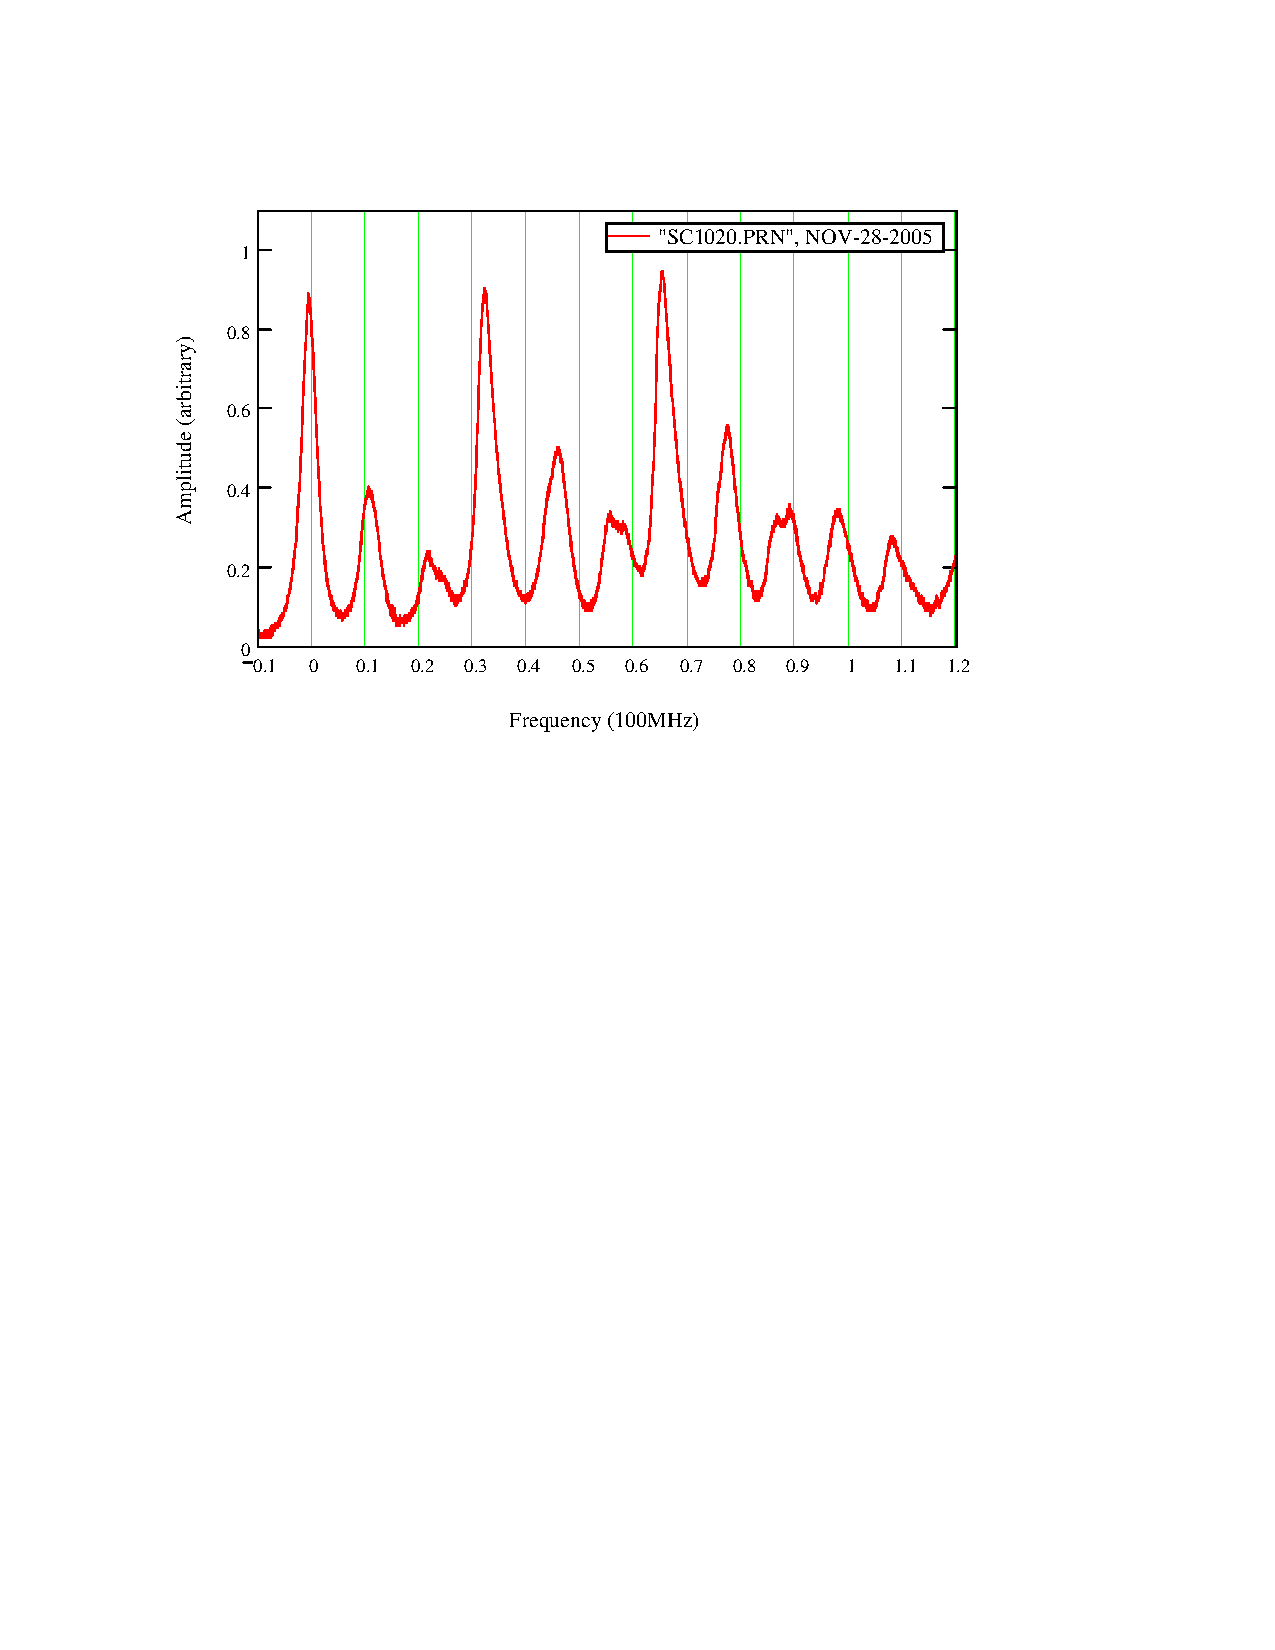
\includegraphics[bb=15 440 489 752]
{near_confocal/near_confocal.pdf}
}
\caption[Green HeNe transmission through a scaned near confocal etalon]{Green HeNe transmission through a scaned near confocal etalon}
\label{near_confocal}
\end{figure}
%----------------------------------------------------------------------------

%----------------------------------------------------------------------------
%----------------------------------------------------------------------------
%bb defines the bounding box for the pdf
%viewport defines the area of the pdf used
%in sidewaysfigure the last entry in bb moves the caption toward/away the pic
%in sidewaysfigure the second entry in bb moves the pic toward/away the caption
%----------------------------------------------------------------------------
\begin{figure}
\scalebox{0.8}[0.8]{
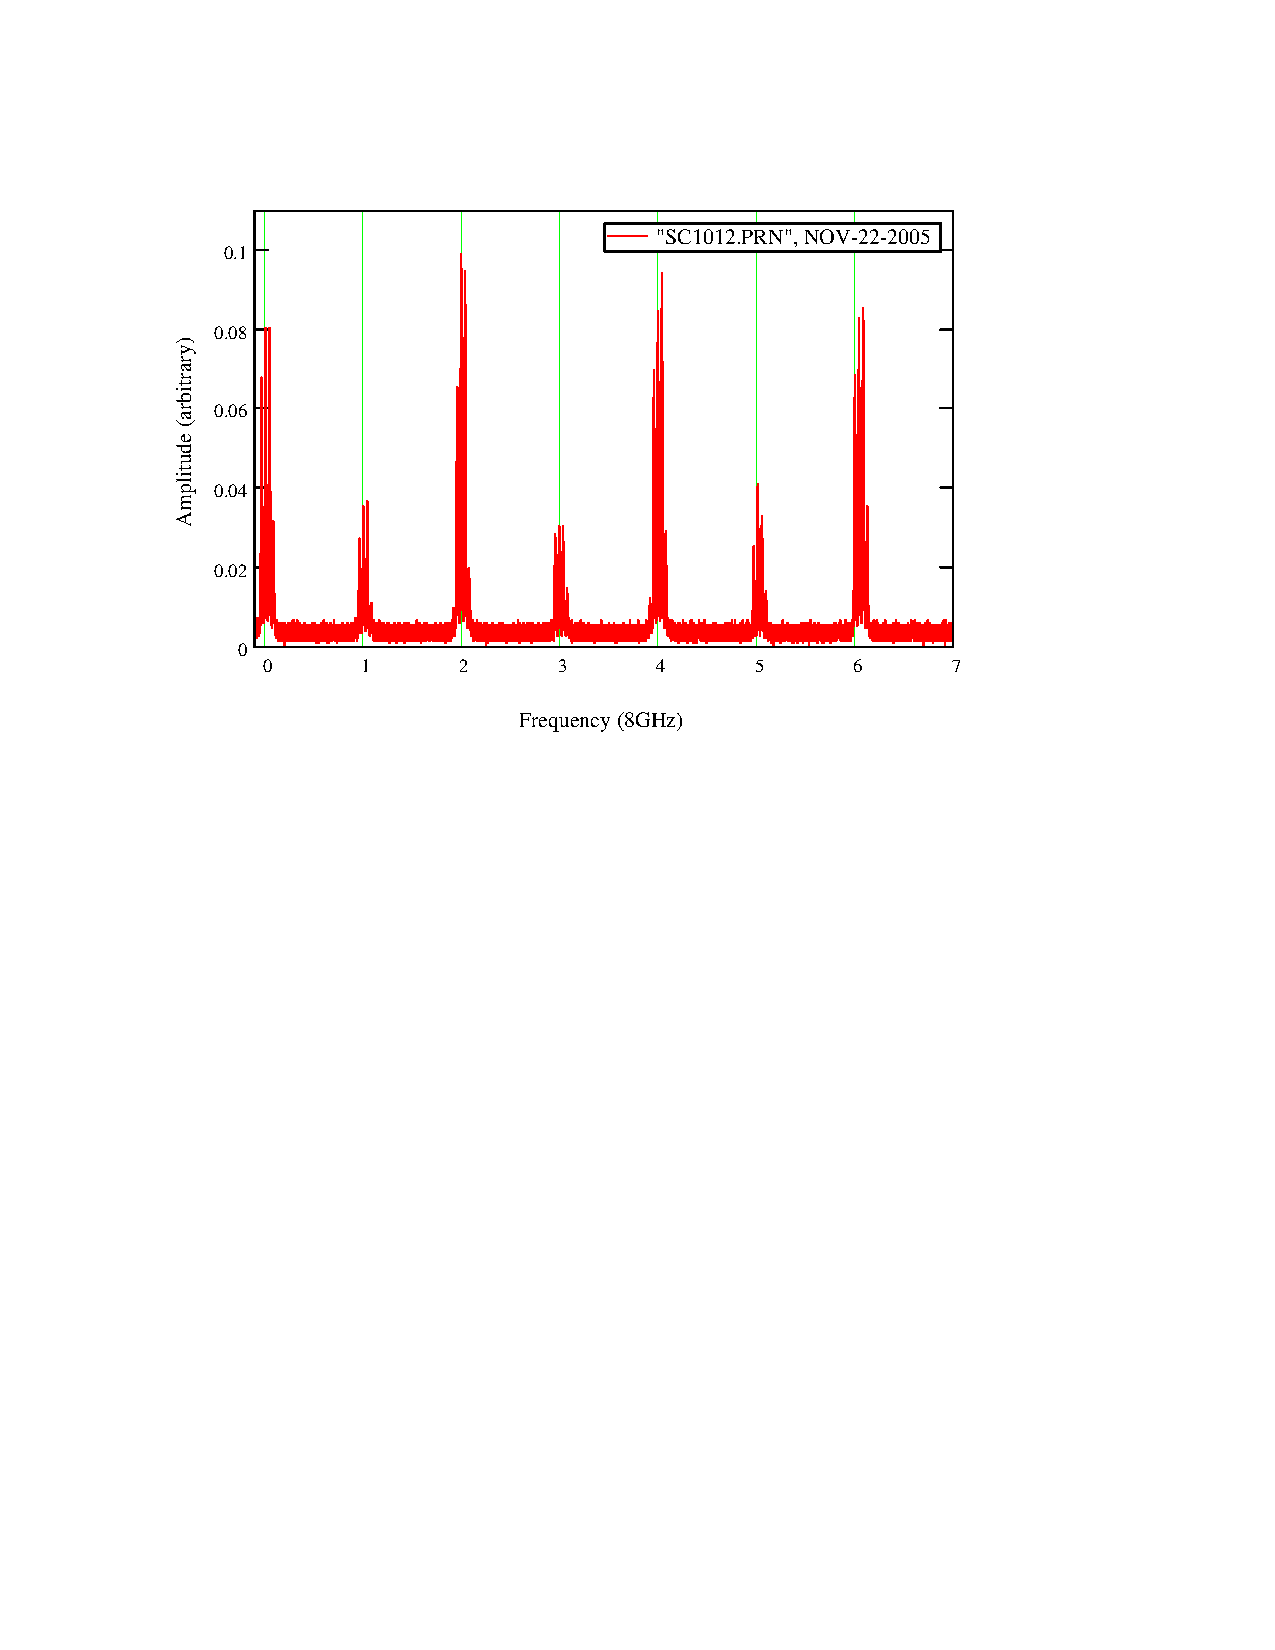
\includegraphics[bb=15 440 489 752]
{confocal_all/confocal_all.pdf}
}
\caption[Green HeNe transmission through a scanned confocal etalon]{Green HeNe transmission through a scanned confocal etalon}
\label{confocal_all}
\end{figure}
%----------------------------------------------------------------------------

%----------------------------------------------------------------------------
%----------------------------------------------------------------------------
%bb defines the bounding box for the pdf
%viewport defines the area of the pdf used
%in sidewaysfigure the last entry in bb moves the caption toward/away the pic
%in sidewaysfigure the second entry in bb moves the pic toward/away the caption
%----------------------------------------------------------------------------
\begin{figure}
\scalebox{0.8}[0.8]{
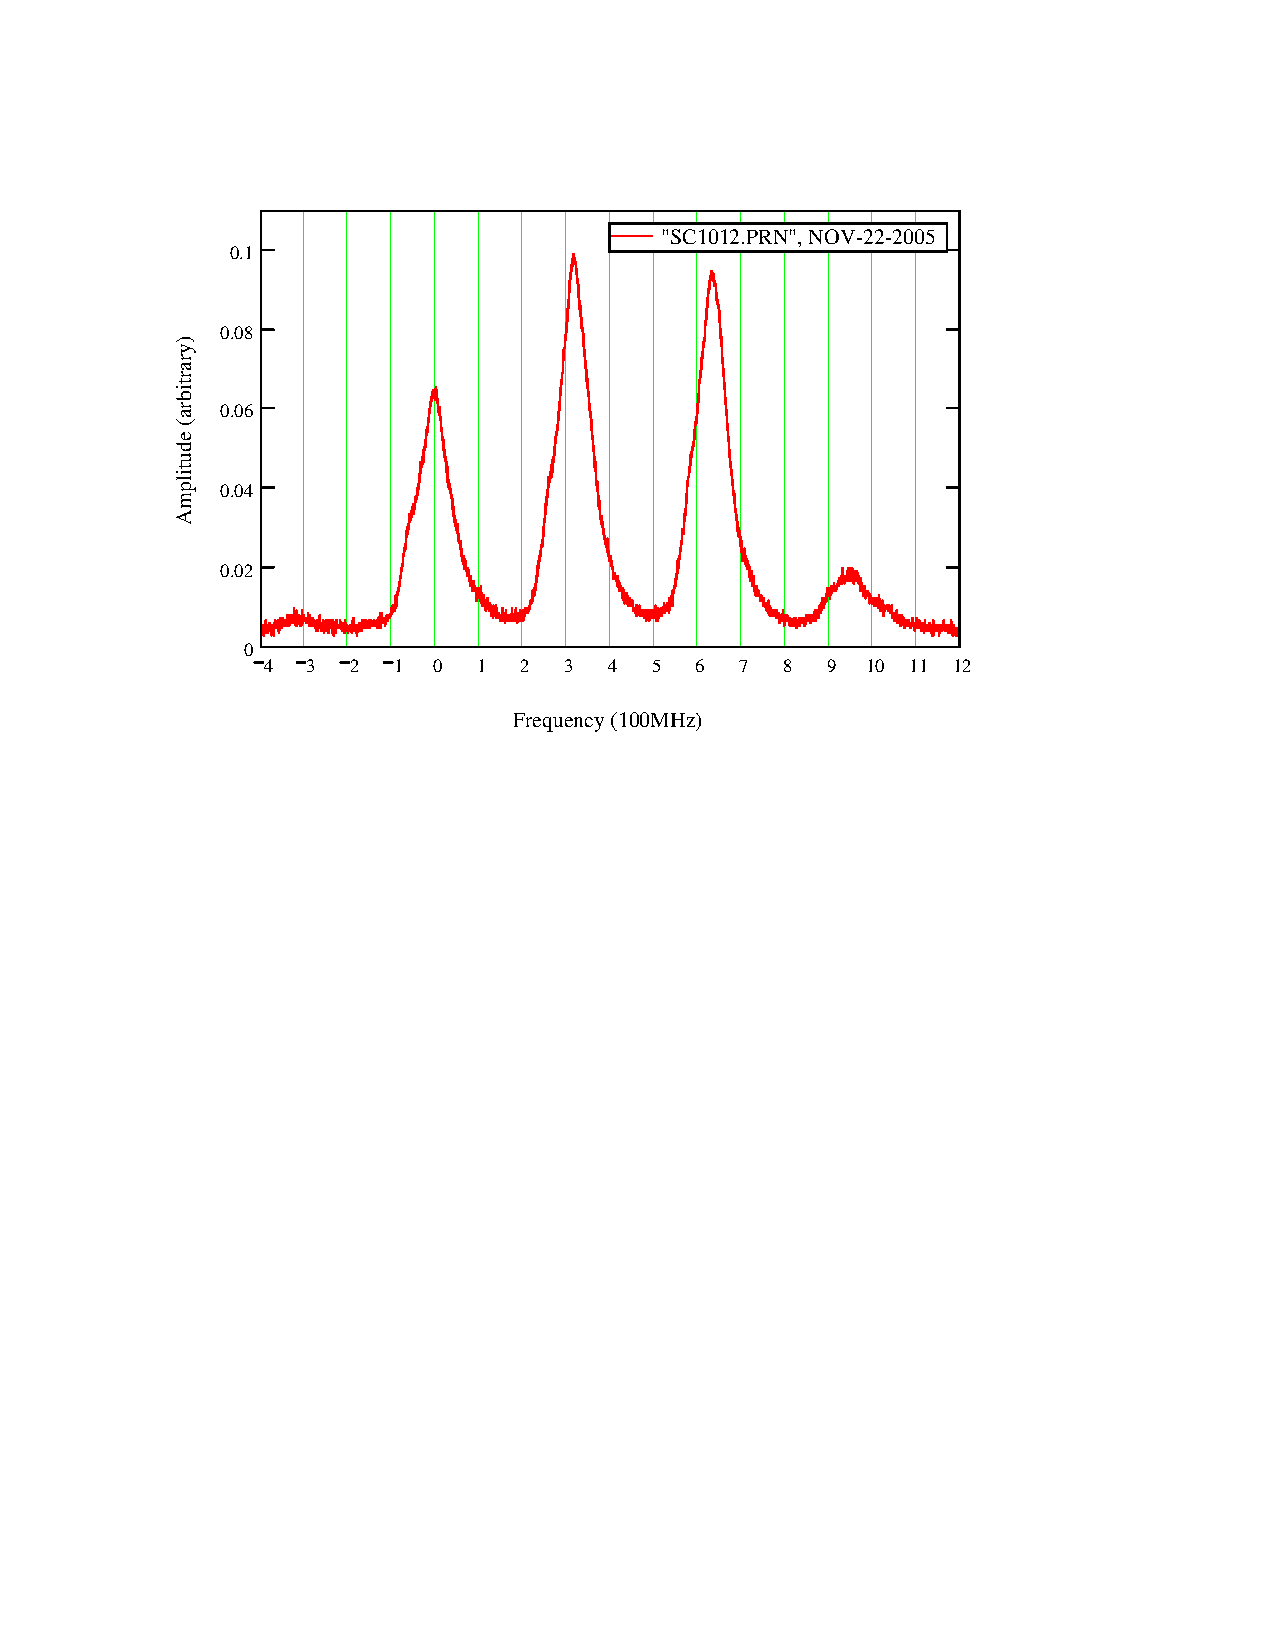
\includegraphics[bb=15 440 489 752]
{confocal_zoom/confocal_zoom.pdf}
}
\caption[Green HeNe transmission through a scanned confocal etalon (zoom)]{Green HeNe transmission through a scanned confocal etalon (zoom). The green HeNe mode spacing is 326 MHz and the etalon mode width is 100 MHz.}
\label{confocal_zoom}
\end{figure}
%----------------------------------------------------------------------------

%----------------------------------------------------------------------------
%----------------------------------------------------------------------------

%----------------------------------------------------------------------------
%----------------------------------------------------------------------------
\section{Single fluorescence line decay}
Decay processes play a major role in this study. The target is assumed to be a relatively unprepared region of atmosphere; thus, in the actual application, we will have little direct control of the parameters that influence the system relaxation. In the experiments leading up to the field demonstration, controlled samples will be used. Here we conduct an initial measurement of the lifetime of a single LIF feature using the ``baked potato'' iodine cell.
\subsection{Pockels cell system integration}
%----------------------------------------------------------------------------
%----------------------------------------------------------------------------
Integration of the Pockels cell into the dye laser system requires the design and assembly of a trigger/delay system used to trigger the YAG pump and delay the activation pulse to the Pockels cell until the incident dye laser pulse arrives at the Pockels cell location (see UH notebook UH--016 pages 56--59). The system consists of three signal generators (HP model 8015A pulse generators), a high voltage DC power supply to charge the Hg pulser (HP model Harrison 6525A), and the associated delay cables and attenuators. The Pockels cell is placed between two polarizing cube beam splitters.
%----------------------------------------------------------------------------
%----------------------------------------------------------------------------

%----------------------------------------------------------------------------
%----------------------------------------------------------------------------
%----------------------------------------------------------------------------
%bb defines the bounding box for the pdf
%viewport defines the area of the pdf used
%in sidewaysfigure the last entry in bb moves the caption toward/away the pic
%in sidewaysfigure the second entry in bb moves the pic toward/away the caption
%----------------------------------------------------------------------------
\begin{figure}
\scalebox{0.8}[0.8]{
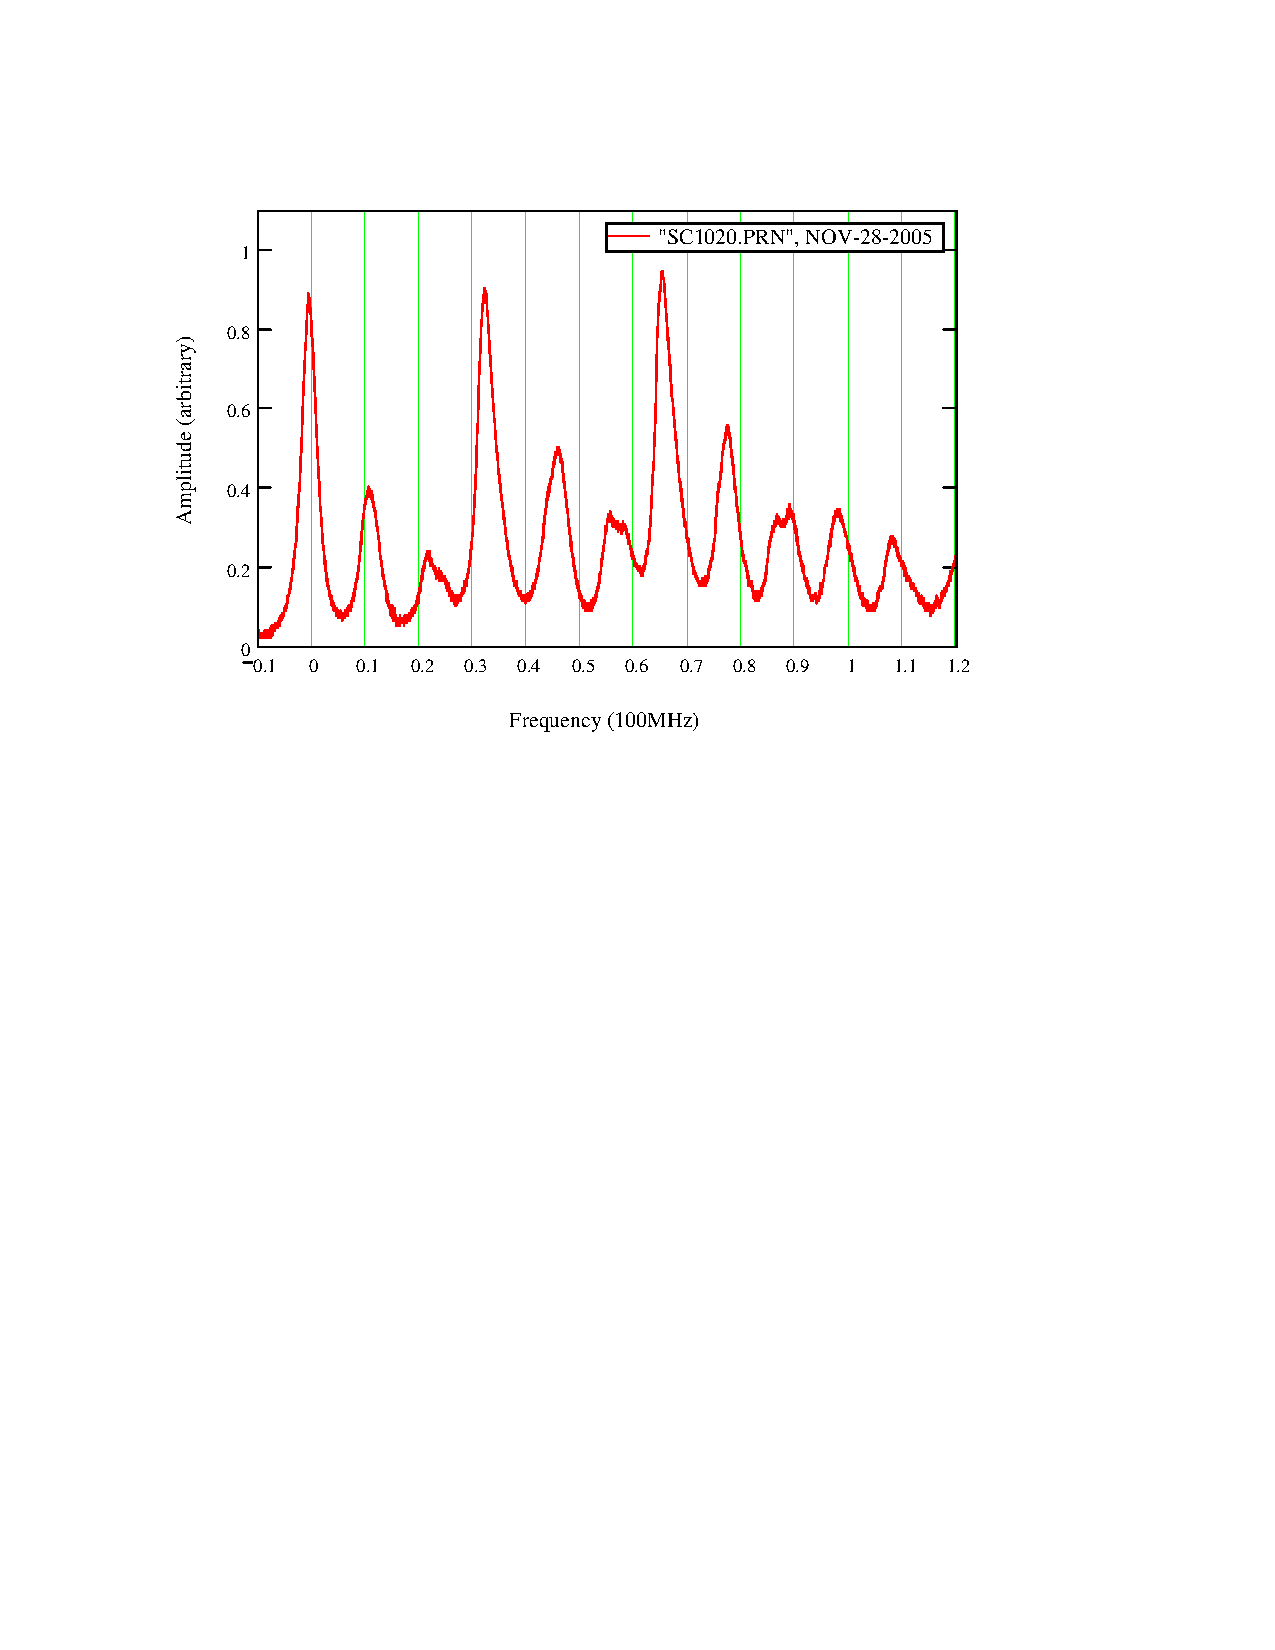
\includegraphics[bb=15 440 489 752]
{near_confocal/near_confocal.pdf}
}
\caption[Green HeNe transmission through a scaned near confocal etalon]{Green HeNe transmission through a scaned near confocal etalon}
\label{near_confocal}
\end{figure}
%----------------------------------------------------------------------------

%----------------------------------------------------------------------------
%----------------------------------------------------------------------------
%bb defines the bounding box for the pdf
%viewport defines the area of the pdf used
%in sidewaysfigure the last entry in bb moves the caption toward/away the pic
%in sidewaysfigure the second entry in bb moves the pic toward/away the caption
%----------------------------------------------------------------------------
\begin{figure}
\scalebox{0.8}[0.8]{
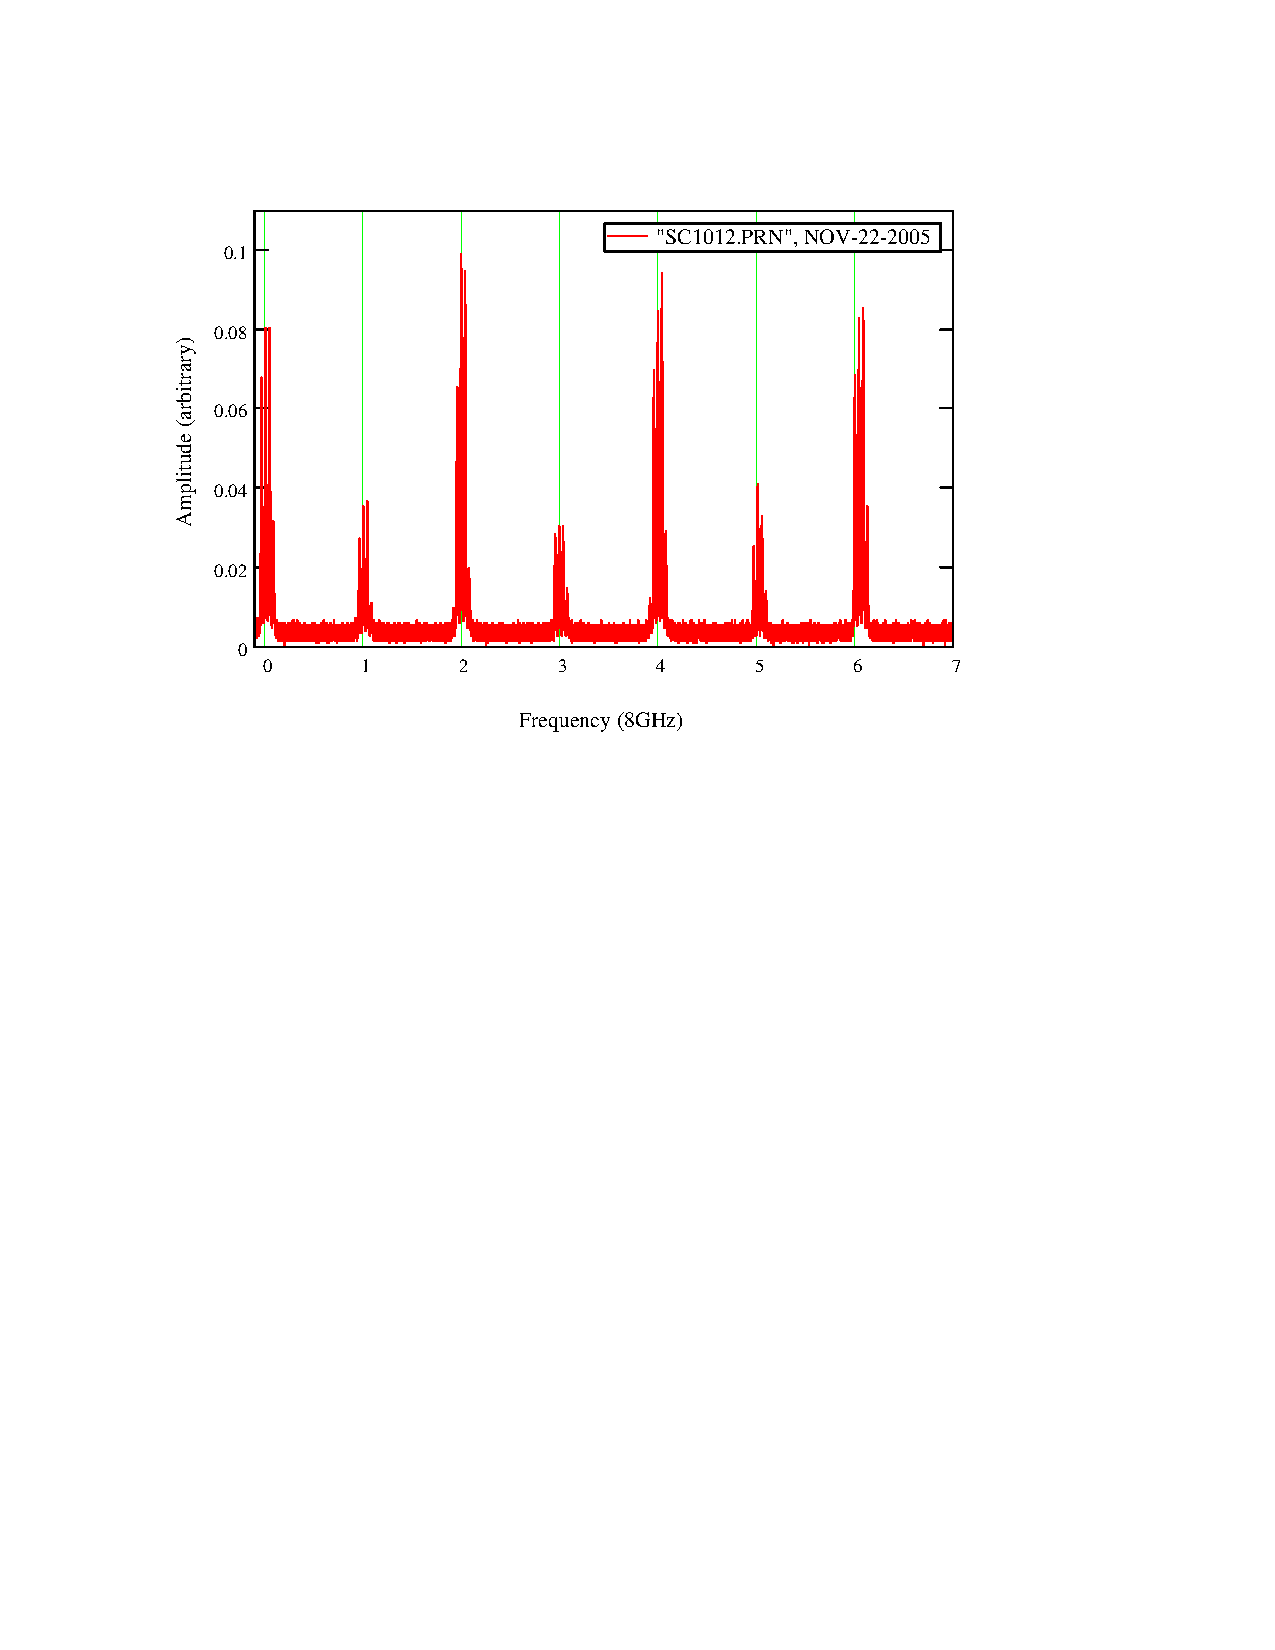
\includegraphics[bb=15 440 489 752]
{confocal_all/confocal_all.pdf}
}
\caption[Green HeNe transmission through a scanned confocal etalon]{Green HeNe transmission through a scanned confocal etalon}
\label{confocal_all}
\end{figure}
%----------------------------------------------------------------------------

%----------------------------------------------------------------------------
%----------------------------------------------------------------------------
%bb defines the bounding box for the pdf
%viewport defines the area of the pdf used
%in sidewaysfigure the last entry in bb moves the caption toward/away the pic
%in sidewaysfigure the second entry in bb moves the pic toward/away the caption
%----------------------------------------------------------------------------
\begin{figure}
\scalebox{0.8}[0.8]{
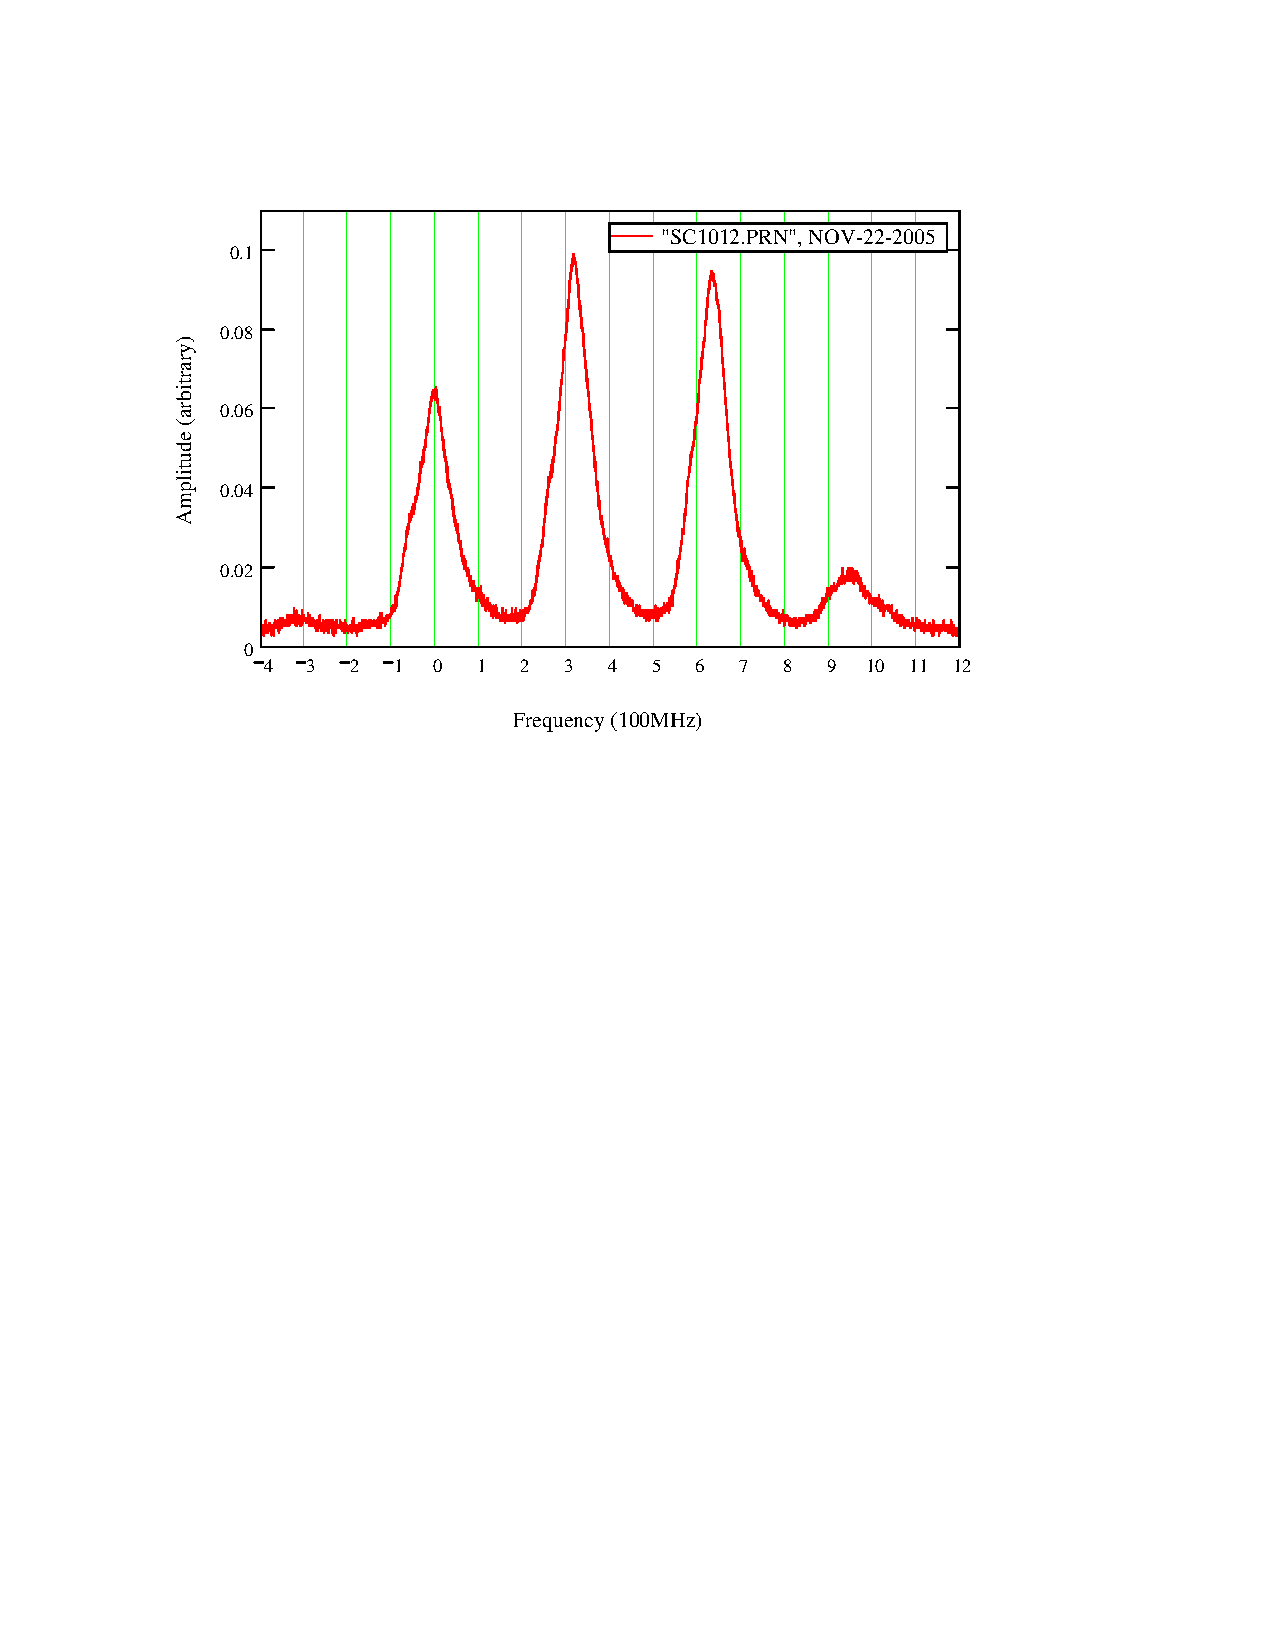
\includegraphics[bb=15 440 489 752]
{confocal_zoom/confocal_zoom.pdf}
}
\caption[Green HeNe transmission through a scanned confocal etalon (zoom)]{Green HeNe transmission through a scanned confocal etalon (zoom). The green HeNe mode spacing is 326 MHz and the etalon mode width is 100 MHz.}
\label{confocal_zoom}
\end{figure}
%----------------------------------------------------------------------------

%----------------------------------------------------------------------------
%----------------------------------------------------------------------------

\subsection{Single fluorescence line decay in molecular iodine}

%------------------------------------------------------------------------------
%------------------------------------------------------------------------------
There are several non-radiative decay mechanisms which can lead to an observed damping of the fluorescence lifetime of a single LIF line. The iodine molecule can dissociate, ionize (once, twice,...), internally decay via a non-optical transition, exchange energy through inelastic collisions, or de-phase through elastic collisions. In Section \ref{density section} we modeled de-phasing through collisions in a stochastic manner. Here we directly measure the observed decay of a LIF line in the ``baked potato'' iodine cell.
%------------------------------------------------------------------------------
%------------------------------------------------------------------------------
%------------------------------------------------------------------------------
%------------------------------------------------------------------------------
%------------------------------------------------------------------------------
%------------------------------------------------------------------------------


%------------------------------------------------------------------------------
%------------------------------------------------------------------------------
The beam line used here is similar to the one described in Section \ref{sample layout} except the attenuators are not used and in its place we use a pair of crossed polarizers (polarizing cube beam splitters) and a Pockels cell. The system has an extinction ratio of about 200:1 (see UH notebook UH-018 page 65) and produces a pulse with a FWHM of about 4 ns. Before the Pockels cell we have about 5.4 mJ, thus after the Pockels cell (heading toward the +750 mm lens) is about 27 uJ. The dye laser is tuned to 535.893 nm (a targeted absorption line) and the monochromator is tuned to capture a single LIF line at 632.9 nm. Again the signal from the PMT at the output of the monochromator is scanned (temporal gate scan) and averaged with a boxcar averager.

The measurement has facilitated the development of the data acquisition system required for lifetime measurements. The boxcar averager works at the 1000 ps gate width setting (it has settings down to 100 ps, but these have not been tried) and the LabView program records the data as a convenient text file. We have also discovered that the intensity fluctuations of the dye laser output introduce unwanted jitter in the position of the trigger relative to the peak -- accurate lifetime measurements will require a way to eliminate the jitter or, better yet, reduce the intensity fluctuations in the input beam. Contamination of the cell may have introduced additional channels through which the iodine can decay. A clean loading method must be developed in order to isolate and measure specific effects on the fluorescence decay.
%------------------------------------------------------------------------------
%------------------------------------------------------------------------------
%------------------------------------------------------------------------------
%------------------------------------------------------------------------------
%------------------------------------------------------------------------------
%------------------------------------------------------------------------------

%----------------------------------------------------------------------------
%----------------------------------------------------------------------------
\section{Aromatic compound LIF}
Iodine is the trial system used to form the computational basis of many of the claims made in this dissertation. The scope of this general study and the development of the experimental equipment go beyond the iodine molecule; this section describes an experiment using naphthalene as a target. Temperature controlled sample cells containing naphthalene have been prepared along with flakes of naphthalene and anthracene. An attempt to observe a multi-photon process in these aromatic samples has led to more equipment development.

%----------------------------------------------------------------------------
%----------------------------------------------------------------------------
%----------------------------------------------------------------------------
%bb defines the bounding box for the pdf
%viewport defines the area of the pdf used
%in sidewaysfigure the last entry in bb moves the caption toward/away the pic
%in sidewaysfigure the second entry in bb moves the pic toward/away the caption
%----------------------------------------------------------------------------
\begin{figure}
\scalebox{0.8}[0.8]{
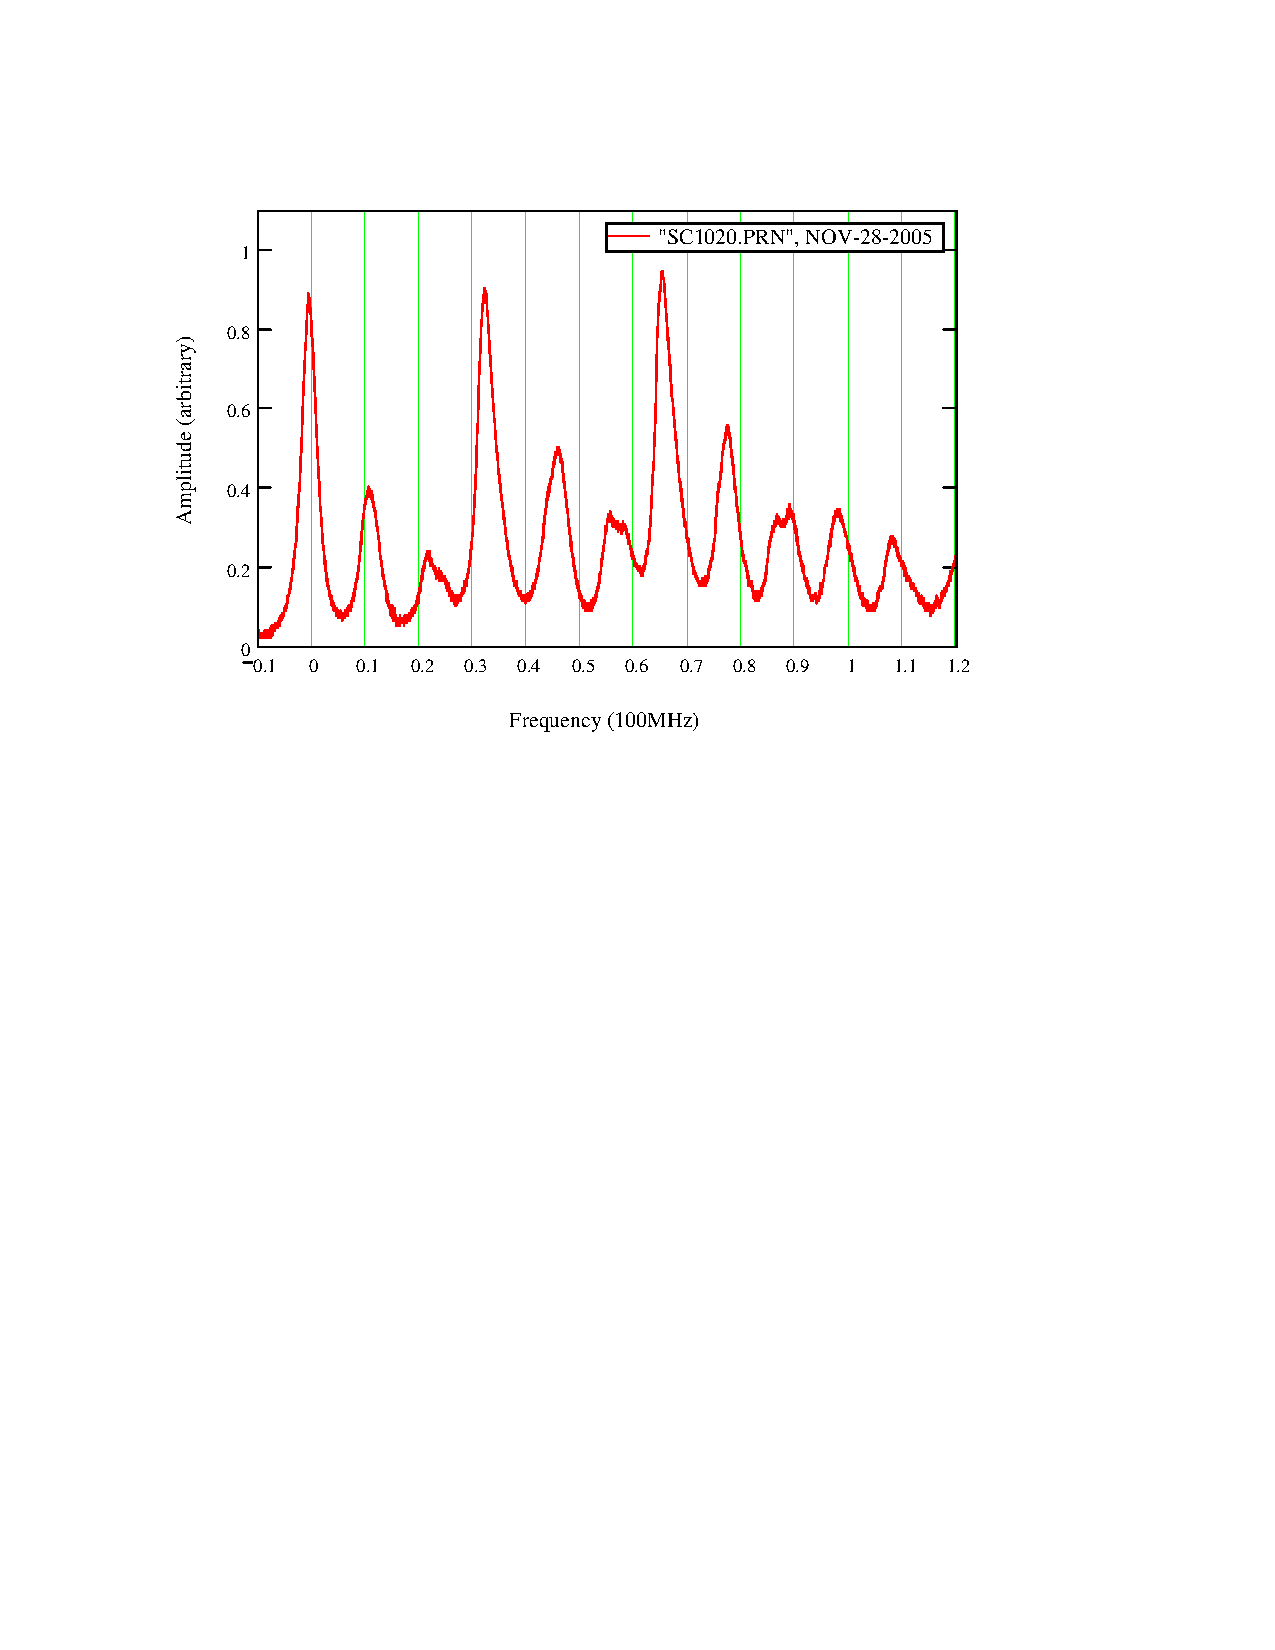
\includegraphics[bb=15 440 489 752]
{near_confocal/near_confocal.pdf}
}
\caption[Green HeNe transmission through a scaned near confocal etalon]{Green HeNe transmission through a scaned near confocal etalon}
\label{near_confocal}
\end{figure}
%----------------------------------------------------------------------------

%----------------------------------------------------------------------------
%----------------------------------------------------------------------------
%bb defines the bounding box for the pdf
%viewport defines the area of the pdf used
%in sidewaysfigure the last entry in bb moves the caption toward/away the pic
%in sidewaysfigure the second entry in bb moves the pic toward/away the caption
%----------------------------------------------------------------------------
\begin{figure}
\scalebox{0.8}[0.8]{
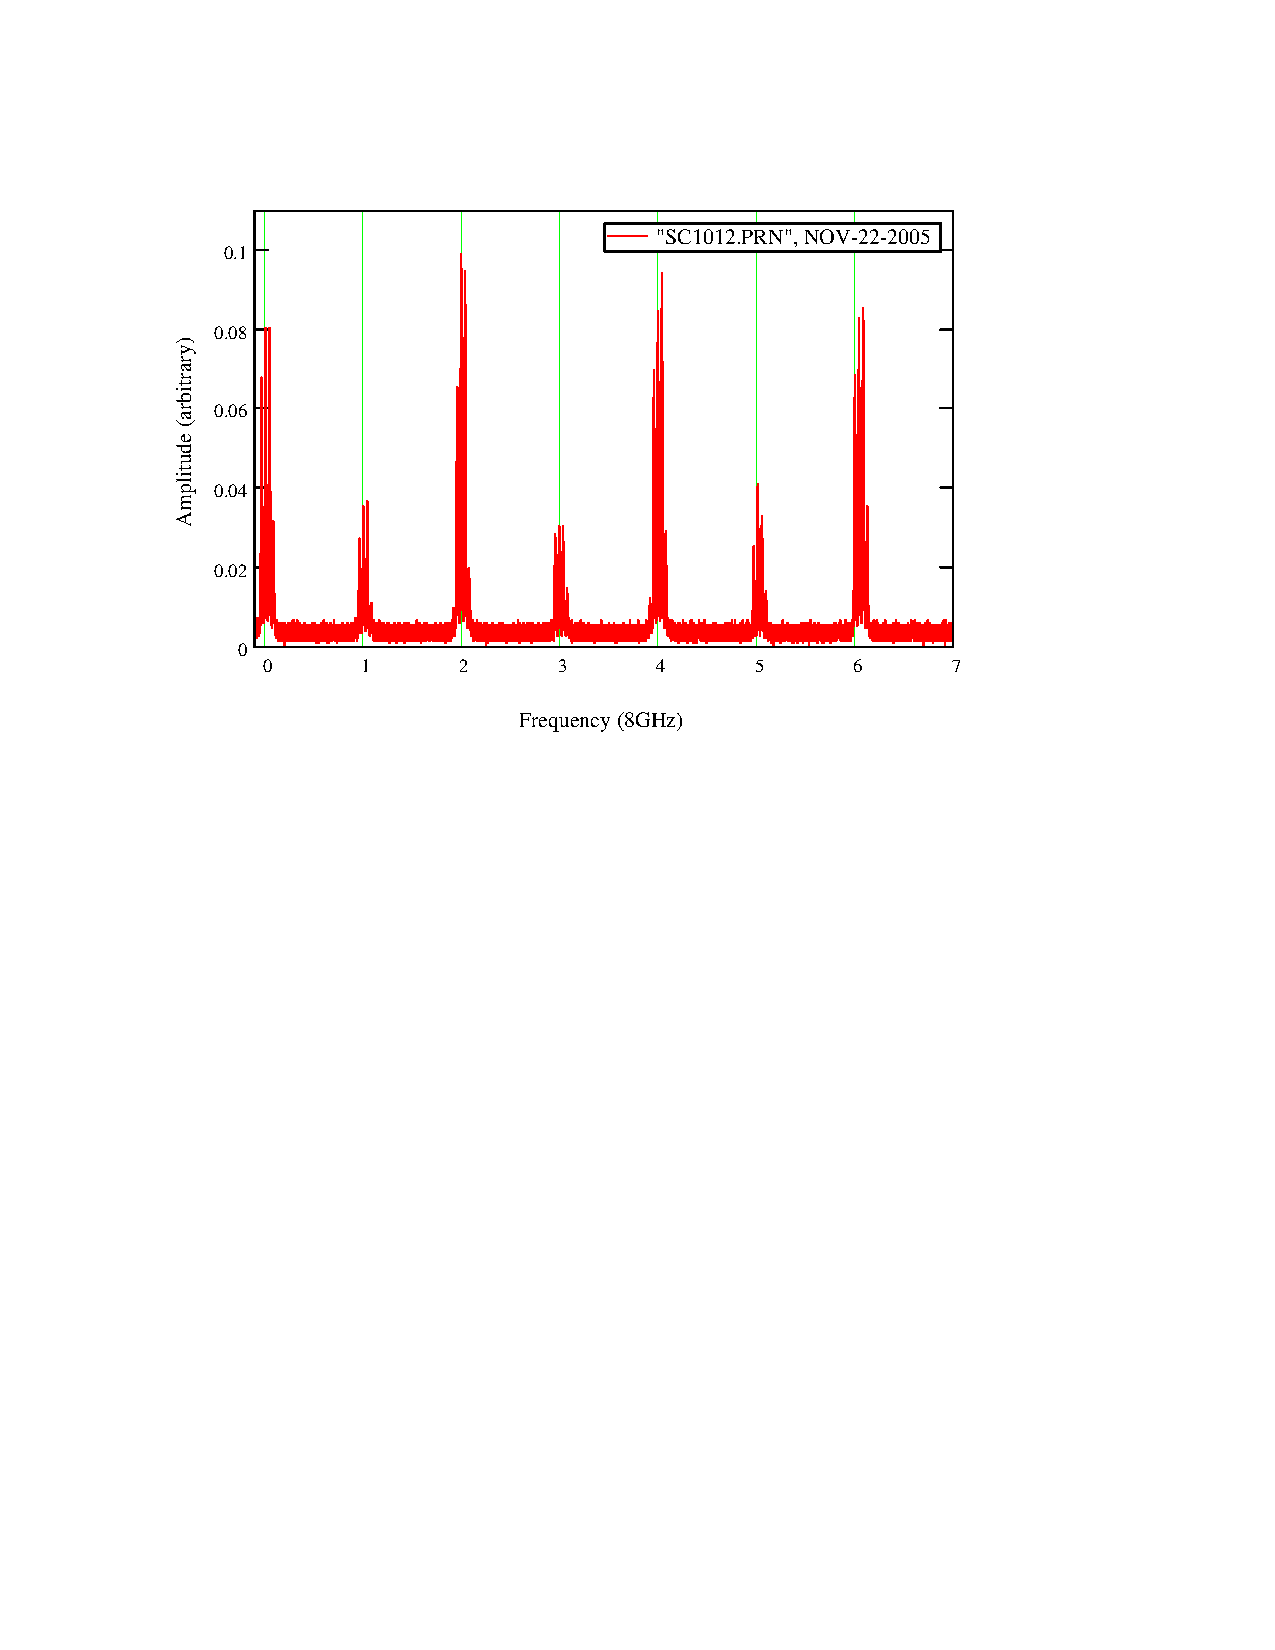
\includegraphics[bb=15 440 489 752]
{confocal_all/confocal_all.pdf}
}
\caption[Green HeNe transmission through a scanned confocal etalon]{Green HeNe transmission through a scanned confocal etalon}
\label{confocal_all}
\end{figure}
%----------------------------------------------------------------------------

%----------------------------------------------------------------------------
%----------------------------------------------------------------------------
%bb defines the bounding box for the pdf
%viewport defines the area of the pdf used
%in sidewaysfigure the last entry in bb moves the caption toward/away the pic
%in sidewaysfigure the second entry in bb moves the pic toward/away the caption
%----------------------------------------------------------------------------
\begin{figure}
\scalebox{0.8}[0.8]{
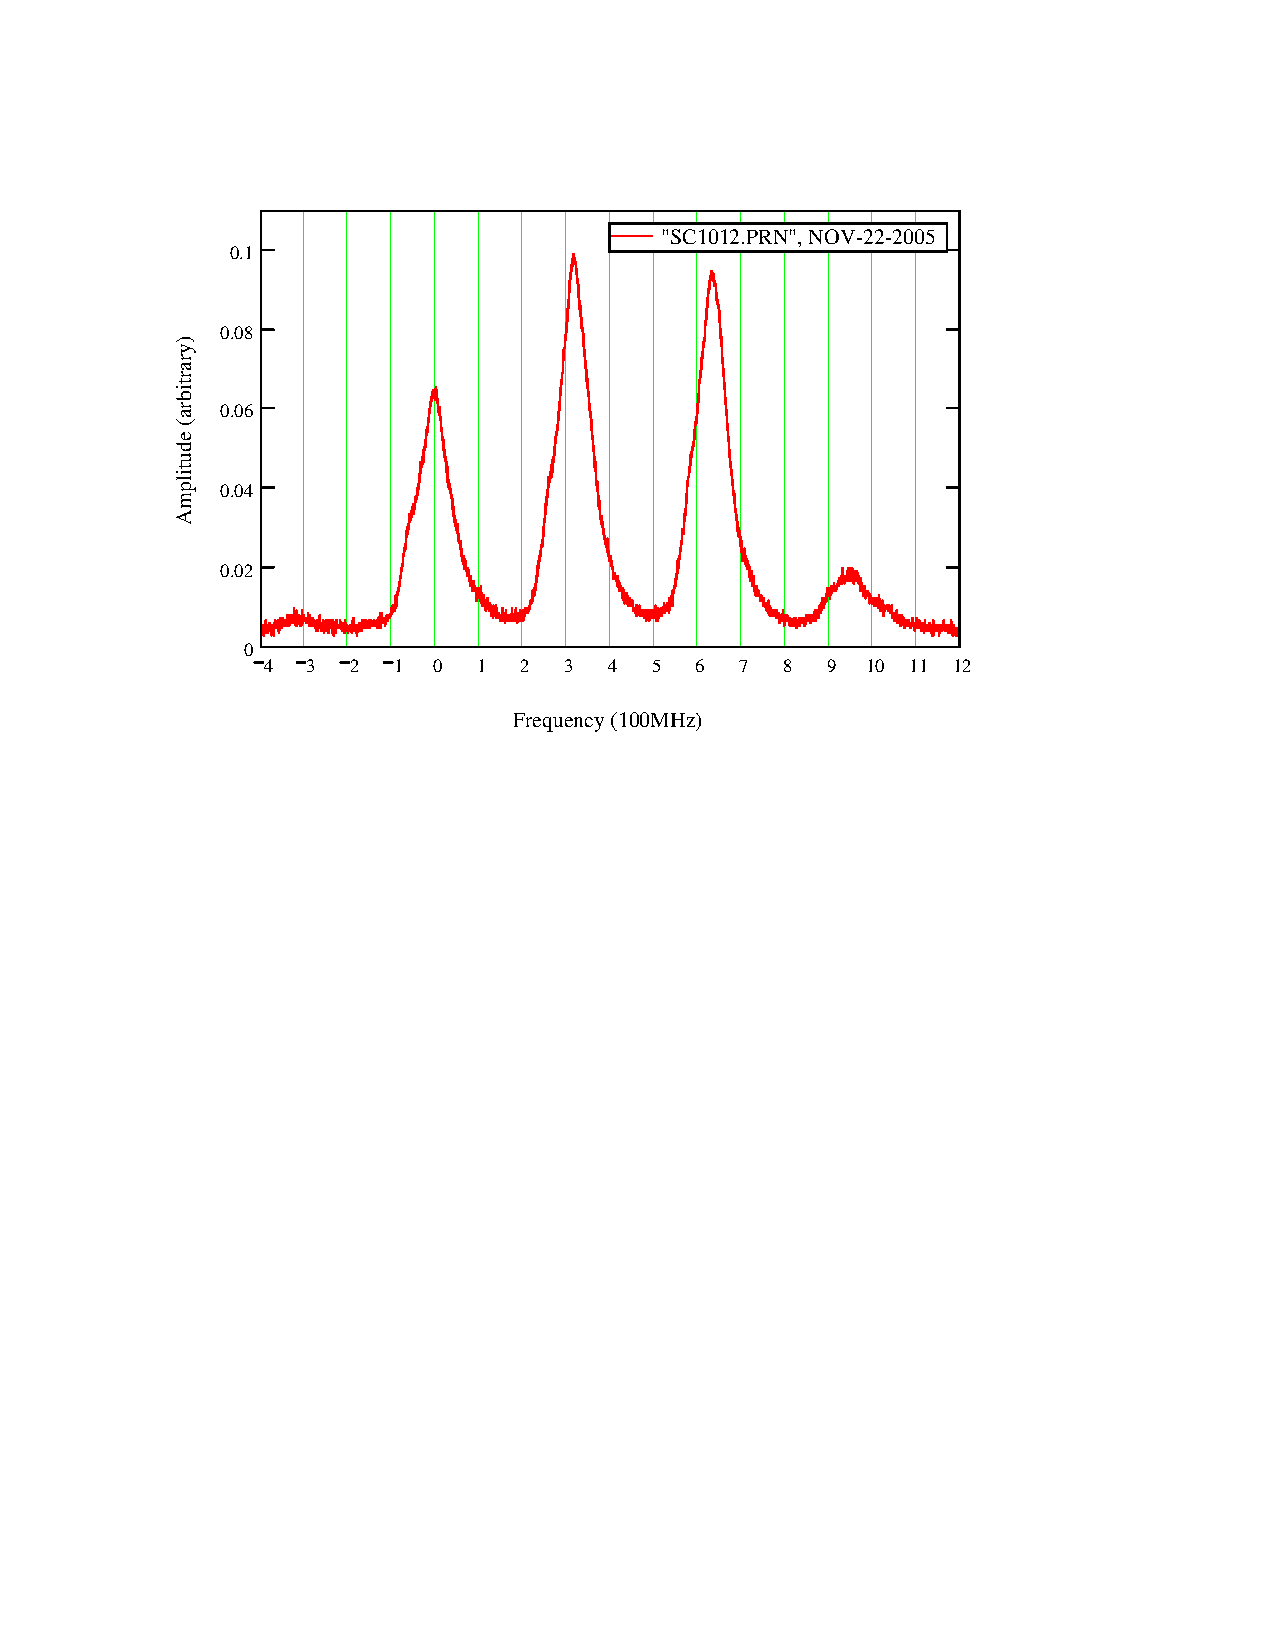
\includegraphics[bb=15 440 489 752]
{confocal_zoom/confocal_zoom.pdf}
}
\caption[Green HeNe transmission through a scanned confocal etalon (zoom)]{Green HeNe transmission through a scanned confocal etalon (zoom). The green HeNe mode spacing is 326 MHz and the etalon mode width is 100 MHz.}
\label{confocal_zoom}
\end{figure}
%----------------------------------------------------------------------------

%----------------------------------------------------------------------------
%----------------------------------------------------------------------------

%----------------------------------------------------------------------------
%----------------------------------------------------------------------------
\section{Conclusion}
%----------------------------------------------------------------------------
%------------------------------Broad objectives------------------------------
%----------------------------------------------------------------------------
This chapter chronicles the stages of laboratory development undergone over the past few years. The main measurements at each stage were used as a guide to develop the equipment and techniques required for demonstration of molecular control in LIDAR systems.
%----------------------------------------------------------------------------
%----------------------------------So what?----------------------------------
%----------------------------------------------------------------------------

As each stage was completed various components of the apparatus were either designed and assembled or evolved to the next generation. After the installation of the PMT at its output the monochromator served each experiment well until the recent aromatic compound measurements. The Hg pulser and Pockles cell system went through various stages of development starting with the initial tests of the Hg pulser on LED's to the integration of the system with the YAG pumped dye laser system during the fluorescence line decay measurements. The software model was tested at each stage from the familiar non-resonant HeNe LIF to pulsed resonant dye LIF. The data acquisition system was built for the first dye laser experiments and has remained relatively unchanged since then. Recently, a calibration issue with the monochromator self scan feature has prompted the need of a second generation of the data acquisition software.
%----------------------------------------------------------------------------
%---------------------------------Synthesize---------------------------------
%----------------------------------------------------------------------------
%----------------------------------------------------------------------------
%----------------------------------------------------------------------------
%----------------------------------------------------------------------------

%----------------------------------------------------------------------------
%----------------------------------------------------------------------------
